\documentclass[11pt,a4paper]{article}
\usepackage{amsmath,amsfonts,amssymb}
\usepackage[shortlabels]{enumitem}
\usepackage{booktabs}
\usepackage{graphicx}
\usepackage{xcolor}
\usepackage{hyperref}
\usepackage{starfont}
\usepackage[
    ]{starfont}
\definecolor{Grey}{rgb}{0.5,0.5,0.5}
\definecolor{Red}{rgb}{1.0,0.0,0.0}

\usepackage{typearea}
\areaset{156mm}{235mm}
\setlength{\parindent}{0pt}

\DeclareSymbolFont{starfontsym}{OT1}{sts}{m}{n}
\DeclareMathSymbol{\mathSun}{\mathord}{starfontsym}{115}
\DeclareMathSymbol{\mathMercury}{\mathord}{starfontsym}{102}
\DeclareMathSymbol{\mathVenus}{\mathord}{starfontsym}{103}
\DeclareMathSymbol{\mathTerra}{\mathord}{starfontsym}{76}
\DeclareMathSymbol{\mathvarTerra}{\mathord}{starfontsym}{108}
\DeclareMathSymbol{\mathMoon}{\mathord}{starfontsym}{100}
\DeclareMathSymbol{\mathvarMoon}{\mathord}{starfontsym}{97}
\DeclareMathSymbol{\mathMars}{\mathord}{starfontsym}{104}
\DeclareMathSymbol{\mathJupiter}{\mathord}{starfontsym}{106}
\DeclareMathSymbol{\mathSaturn}{\mathord}{starfontsym}{83}
\DeclareMathSymbol{\mathUranus}{\mathord}{starfontsym}{70}
\DeclareMathSymbol{\mathvarUranus}{\mathord}{starfontsym}{65}
\DeclareMathSymbol{\mathNeptune}{\mathord}{starfontsym}{71}
\DeclareMathSymbol{\mathPluto}{\mathord}{starfontsym}{74}
\DeclareMathSymbol{\mathvarPluto}{\mathord}{starfontsym}{72}


\renewcommand\floatpagefraction{0.8}
\renewcommand\topfraction{1}
\renewcommand\bottomfraction{0.9}
\renewcommand\textfraction{0.0}


\definecolor{arsenic}{rgb}{0.0666, 0.0666, 0.10588}
\definecolor{text}{rgb}{0.8039, 0.8392, 0.95686}
\pagecolor{arsenic}
\color{text}

\begin{document}

\title{Astrophysik Zusammenfassung}

\author{}

\date{}

\maketitle

\tableofcontents

\newpage


\section{useful stuff}
\begin{align*}
    1 W &= 10^7 \frac {erg} s \\
    1'' &= \frac \pi {180 \cdot 3600}\\ 
    d &= \frac 1 p \\
\end{align*}
\section{Astronomical Principals}
\subsection{Refraction}
The speed of light in a medium is lower by the refractive index n:
\begin{align*}
   c_m = \frac c n 
\end{align*}
Refractive index: 
\begin{align*}
    n_0 sin \alpha_0 = ... &= n_\infty sin \alpha_\infty \\ 
    n_\infty sin \alpha_\infty &= sin (\alpha_0 + \Delta \alpha) = sin \alpha_0 cos \Delta \alpha + cos \alpha_0 sin \delta \alpha\\ 
    \Delta \alpha &\ll 1  \\ 
    \rightarrow sin \Delta \alpha \approx \Delta \alpha, cos \Delta \alpha \approx 1 \\ 
    n_0 sin \alpha_0 &= sin \alpha_0 + \Delta \alpha cos \alpha_0 \\ 
    \rightarrow \Delta \alpha &= tan \alpha_0 (n_0 - 1)
\end{align*}
Refraction also depends on wavelength/frequency.
\subsection{Seeing}
Turbulence causes the density and temperature to shift stochastically $\rightarrow$ path of light is distorted.
\begin{center}[ht!]
    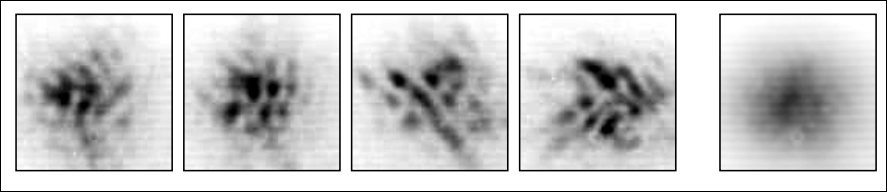
\includegraphics[width=\linewidth]{screenshot_2024-01-12-192223.png}
\end{center}
\paragraph{Solutions}
\begin{itemize}
    \item speckle interferometry:  \\ 
        interferometric combination of short-exposure speckle images to obtain a diffraction-limited resolution image; works best on bright objects
    \item Adaptive optics: \\ 
        correct the shape of the mirror as determined from millisecond-measured
wave-front distortions of a bright star in the FoV or an artificial guide star (laser).
\end{itemize}
\subsection{Atmospheric absorption}
\begin{center}[ht!]
    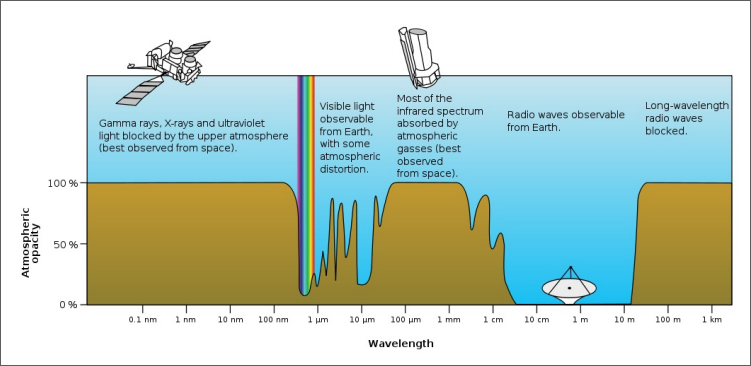
\includegraphics[width=\linewidth]{screenshot_2024-01-12-190242.png}
\end{center}
$\rightarrow$ two main windows: Optical, Radio
Absorption effects:
\begin{itemize}
    \item Reflection of long radio waves by the ionosphere 
    \item Photoabsorption in the IR by $O_3, O_2, H_2 O, CO_2,...$
    \item Scattering and Ionization in the UV spectrum
    \item Photoabsorption in the X-Ray spectrum
\end{itemize}
Optical Depth: \\ 
The height $\tau = 1$ where the original radiation Flux $F_0$ has decreased to F = $\frac 1 e F_0$.
\begin{align*}
    F = F_0e^{-\tau} 
\end{align*}
\subsection{very-high-energy gamma-ray astronomy}
Process: 
\begin{itemize}
    \item VHE $\gamma$-ray photon hits atmosphere 
    \item pair production in the vicinity of the nucleus of an atmospheric molecule
    \item electron-positron pair emits Bremstrahlung because of Coulomb interactions with other atoms
    \item more pair production (shower cascade)
    \item particle speeds exceed the speed of light in the medium
    \item Cherekov radiation is emitted
\end{itemize}
\subsection{The basics of telescopes}
Purpose is 1. to collect light of faint objects and 2. to resolve small features.
This leads to the two main criteria of a Telescope: 1. Sensitivity and 2. Angular resolution.

Telescopes are used to: 
\begin{itemize}
    \item Make images, today with Charge Coupled Devices [CCDs], historically with film
    \item to measure spectra, by using spectrograph's
    \item to measure brightness, by using Photometers (often CCDs in the optical to X-ray) and Bolometers in the Radio regime
\end{itemize}
\subsection{Telescope types}
There are two main types of telescopes. 
\begin{itemize}
    \item Refractors: using lenses \\ 
        Size is limited to $\approx$ 1 m as the lens cannot be supported from the back.\\ 
        not really used anymore.
    \item Reflectors: using Mirrors  \\ 
        Diameter of up to 10 m.
\end{itemize}
\begin{center}[ht!]
    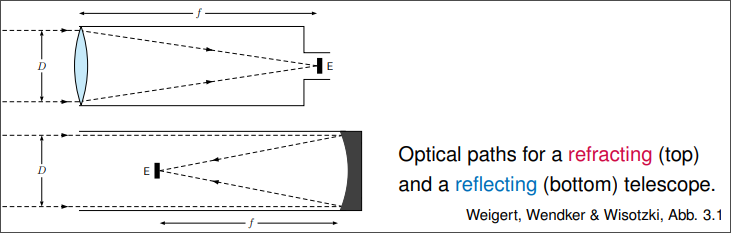
\includegraphics[width=\linewidth]{screenshot_2024-01-13-191726.png}
    \text{Focal length f}
\end{center}
Mirrors have to be parabolic to focus light into one point.
This isnt the case with Schmidt telescopes.
They use a spherical mirror with a correction plate to correct spherical aberration and are used to conduct surveys due to their larger fov.
\begin{center}[ht!]
    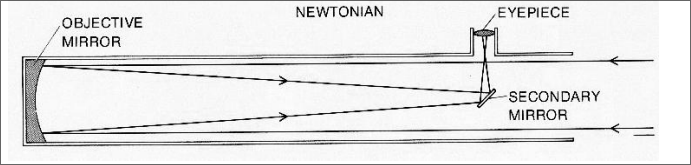
\includegraphics[width=\linewidth]{screenshot_2024-01-13-192049.png}
    \text{Newtonian telescope (reflector)}
\end{center}
\begin{center}[ht!]
    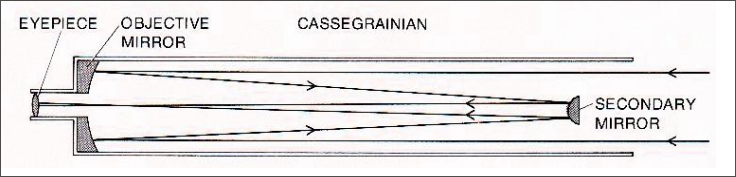
\includegraphics[width=\linewidth]{screenshot_2024-01-13-192236.png}
    \text{Cassegrian Telescope, can be shorter than Newtonian, usually used nowadays}
\end{center}
\subsection{Diffraction}
The wave nature of light causes a interference pattern caused by diffraction of optical elements in the telescope.
The diffraction is minimal for:
\begin{align*}
    \theta = \frac{1.22 \lambda}{d} 
\end{align*}
where d is the diameter.
\subsection{Angular resolution}
The angular resolution is affected by three effects: 
\begin{itemize}
    \item Seeing 
    \item chromatic/spherical Aberration (light of different wave lengths gets dispersed by different amounts)
    \item Diffraction 
\end{itemize}
Resolution is defined as a telescopes ability to separate two point like sources of light.
For this we ca use the Rayleigh criterion for resolution: \\
The maximum of the diffraction pattern of one source must fall
into minimum of the diffraction pattern of another source.
\begin{align*}
    \theta = \frac{1.22 \lambda}{d}  = \frac {12''}{D/1cm}
\end{align*}
\subsection{Radio Telescopes}
Radio telescopes come in many different shapes and sizes.
They do however have to be big to achieve good resolution.
They are often steerable parabolic based, but also phased or interfemotrie approaches exist too.
\begin{center}
    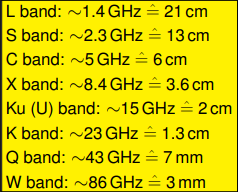
\includegraphics[width=0.6\linewidth]{screenshot_2024-01-13-195458.png}
\end{center}
15MHz to 40 GHZ largely transparent with a dip at 22 GHz due to water vapor.
High-frequency windows at ~3 mm (65–115 GHz), ~2 mm (125–180 GHz), and
~1.2 mm (200–300 GHz) and submillimeter windows (ALMA bands).

\subsection{X-Ray telescopes}
Angle necesery for reflection: 
\begin{align*}
    \theta = 5.6' \sqrt{\frac{\rho}{1 g/cm^3}} \frac \lambda {1nm} 
\end{align*}
So for metallic mirrors $\theta \sim 1deg$.

Higher density materials lead to higher $\theta$ (z.b. Gold or iridium).
Total reflection only works well in soft X-rays due to $\lambda$ leading to the effective area falling.

To obtain manageable focal lengths:
\begin{center}
    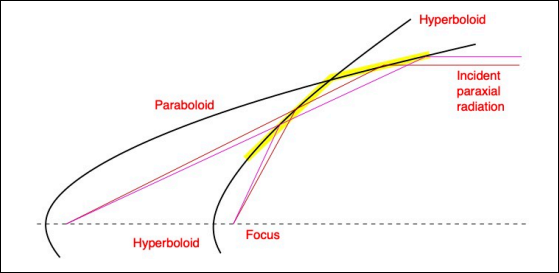
\includegraphics[width=0.6\linewidth]{screenshot_2024-01-13-200712.png}
\end{center}
But this does lead to a small collection area.
\subsection{Position on earth}
\begin{center}
    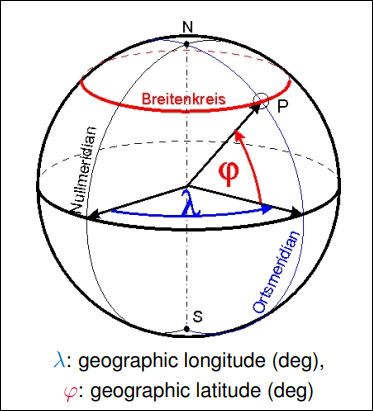
\includegraphics[width=0.6\linewidth]{screenshot_2024-01-13-200901.png}
\end{center}
$\lambda = 0$ defined at Greenwich
\subsection{Horizon System}
\begin{center}
    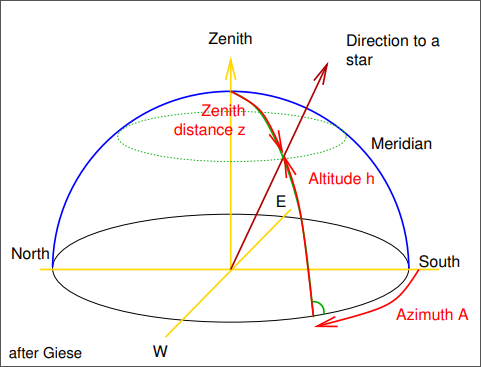
\includegraphics[width=0.6\linewidth]{screenshot_2024-01-13-201929.png}
\end{center}
Two coordinates to define a direction:
Azimuth A: angle SWNE and Altitude h angle towards zenith (or zenith distance 90deg - h). 
\subsection{Equatorial system}
\begin{center}
    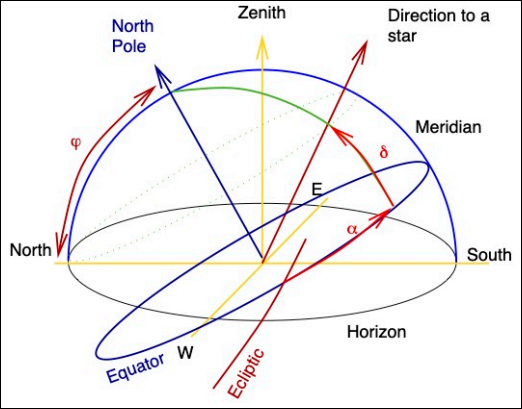
\includegraphics[width=0.6\linewidth]{screenshot_2024-01-13-202353.png}\\
\end{center}
$\alpha$ right ascension, distance from vernal equinox to star \\ 
t hour angle measured from south to west depends on location on earth and time.
$\delta$ Declination angle from equator to star(Moving Equatorial system). 
Siderial time ?
\section{Solar System}
\begin{align*}
    \vec F &= -Gm_1m_2 \frac {\vec r } {r^3} \\ 
\vec F &= m_2  \ddot \vec r_2 \\
\end{align*}
$\rightarrow$ equation of motion: 
\begin{align*}
    m_2  \ddot \vec r_2 &= -Gm_1m_2 \frac {\vec r } {r^3} \\
\end{align*}
    \text {For sun:} 
\begin{align*}
    m_1  \ddot \vec r_2 &= +Gm_1m_2 \frac {\vec r } {r^3} \\
\end{align*}
    \text {Relative Orbit: (Subtract the equations)}
\begin{align*}
    \ddot \vec r &= G(m_1 + M-2) \frac {\vec r } {r^3}
\end{align*}
\subsection{Keplers Laws}
\begin{center}
    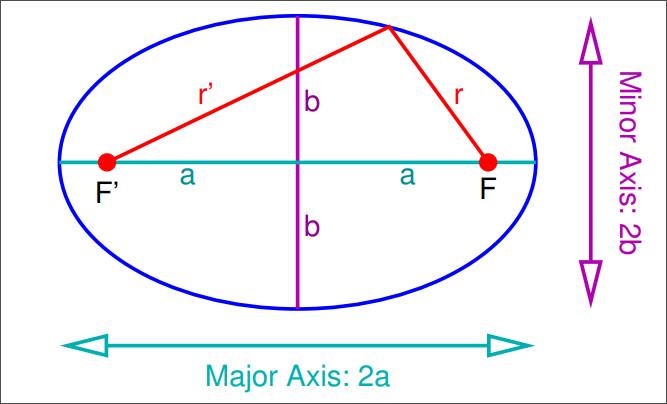
\includegraphics[width=0.6\linewidth]{screenshot_2024-01-14-181441.png}
\end{center}
Ellipse defined as:
\begin{align}
   r + r' = 2a 
\end{align}
where a is the semi-major axis. 
\begin{center}
    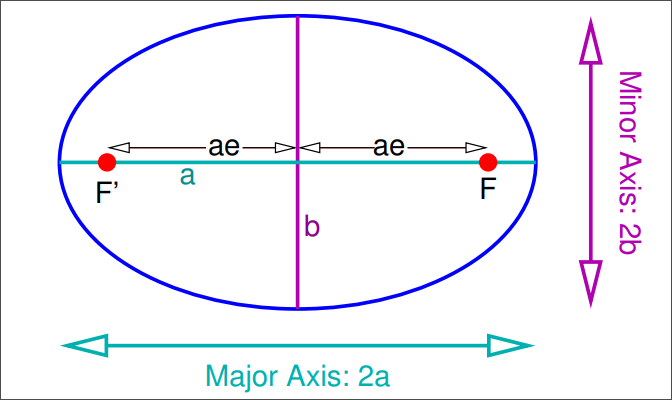
\includegraphics[width=0.6\linewidth]{screenshot_2024-01-14-182015.png}
\end{center}
\newpage
Eccentricity is the factor a has to be multiplied by to get to the focal points. 
\begin{center}
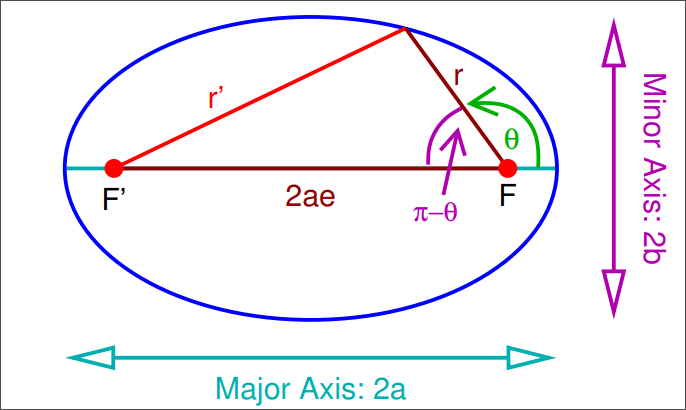
\includegraphics[width=0.6\linewidth]{screenshot_2024-01-14-182509.png}
\end{center}
\begin{align}
    r = \frac{a(1-e^2)}{1+ecos\theta } 
\end{align}
with $\theta$ being the true anomaly.\\
The Perihelion is the closest point to an object, while the aphelion is the farthest point.
\begin{align*}
    d_p &= a - ae = a(1-e) \\  
    d_a &= a + ae = a(1+e) \\  
\end{align*}


\begin{enumerate}
    \item The orbits of the planets are ellipses and the Sun is at
one one of the focal points of the ellipse. 
\item The radius vector to a planet sweeps out equal areas
in equal intervals of time. 
\item The squares of the periods of the planets, P, are proportional to the cubes of the semimajor axes.
    \begin{align*}
        P^2 &= \frac{4 \pi^2}{G (m_1 +M_2)} R^3 \\ 
        \frac {P^2}{ a^3} &= \frac {4 \pi ^2 } {GM} = const.
    \end{align*}
\end{enumerate}
\subsection{Three body Problem}
No analytical solution, but solvable if restricted to two bodys.
This leads to langrange points:
\begin{center}
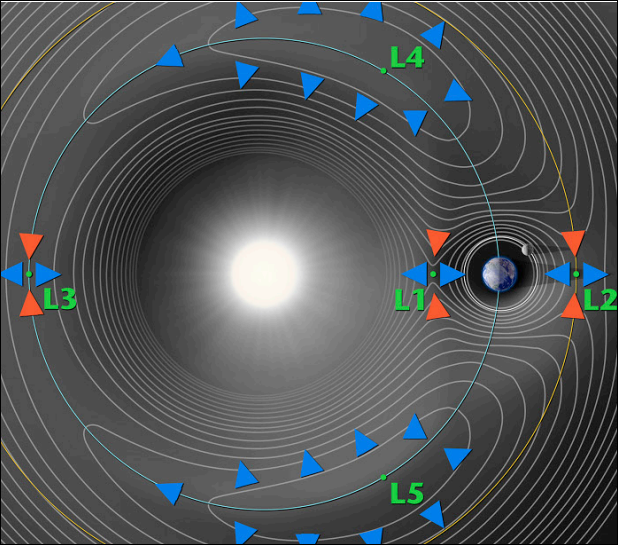
\includegraphics[width=0.5\linewidth]{screenshot_2024-01-14-183945.png}\\
\end{center}
L1,L2,L3 are unstable while L4 and L5 are stable.
\subsection{Precession and Nutation}
The orbital planes of the sun and moon are not in line with the equator.
This leads to them exerting a force onto the earth. 
This leads to two distinct effects: 
\begin{itemize}
    \item luni-solar precession: \\ 
        Earth’s axis rotates around pole of ecliptic once every
25800 years
\item nutation: \\ 
    "Wobble" with 18 year period.
\end{itemize}
\subsection{N-Body systems}
Motion of the i-th object:
\begin{align*}
    m_i \ddot \vec r &= \sum_{k=1}^N \frac{Gm_im_k}{r_{i,k}^2} \frac {\vec r_i - \vec r_k}{r_{i,k }}
\end{align*}
This has no closed solutions, Analytical approach with perturbation theorie:
\begin{enumerate}
    \item Assume two body motion around Sun for all planets
    \item Evaluate force based on this motion.
    \item Update positions with this “perturbation”.
    \item Iterate (i.e., goto step 2) 
\end{enumerate}
This yields two kinds of perturbations: 
 \begin{enumerate}
     \item Periodic perturbations leading to sin and cos- functions 
     \item secular perturbations leading to polynomial terms and describe long term effects (includes time in calculations)
 \end{enumerate}
 The analytical approach is tedious and does not converge for large time scales.\\ 
 $\rightarrow$ numerical solutions.
\subsection{Comets}
Their orbits can be off axis and very eccentric.
They have a wide range of orbits between 2AE and $2 \cdot 10 ^4 $ AE.
The likely origin of a lot of comets is the Oort cloud. 
They are small with a radius of about 1-100km and a low mass. 
They are comprised of ice, eg ($H_20, NH_3, ...$) dust and small rocks. 

Near the perihel the comets tend to gas out due to ice melting. 
This leads the formation of the coma. 
The tail of a comet is formed by interactions of sunlight with the coma.
The difference in pressures leads to the formation of the dust tails by radiative pressure and the ion tail by solar wind.
The earth passing this tail can lead to meteor showers. 
The radiation pressure is given by: 
\begin{align*}
    F_{rad} &= \frac {\rho L_{\odot}}{4 \pi r^2 c}
\end{align*}
With $\rho$ being the cross-section of a particle. \\
The angle caused by the solar wind is given by: 
\begin{align*}
    tan \phi &= \frac {v_\theta}{v_{sw} -v_r} 
\end{align*}
With $v_{sw}$ being the velocity of a particle from the sun and $v_r, v_\theta$ the radial and transversal velocity of the comet. 
The angle is typically below five degree. 
\subsection{solar Corona}
The corona is a part of the suns atmosphere that can be seen during a solar eclipse with the eye as sunlight is scattered of electrons in streamers. 
The plasma in the corona has a temperature of above $10^6$ K which can be seen in the EUV and X-Ray regimes. 

Coronal holes are darker regions in the X-ray regions that are left behind by magnetic filed lines opening up to the interplanetary medium leading to particles escaping. 
This can be seen as solar wind.

At earth the solar wind has a density of 6-7 protons per cubic centimeter and a temperature of $10^5$ Kelvin with a speed of around 400 kms.
It is mostly comprised of protons and electrons with some heavier ions.

Reconnection of magnetic field lines can lead to Coronal mass ejections (CMEs) with particle speeds between 50 kms and 2500 kms. 

Solar wind is a supersonic flows in the IM. This leads to discontinuities when encountering a planet. 
This leads to shocks. 
A shock front is a discontinuity across which there is a steady flow of
mass, momentum, and energy.
\subsection{Planets}
A planet is a celestial body, that: 
\begin{enumerate}
    \item Orbits the sun
    \item has sufficient mass to assume hydrostatic equilibrium
    \item has cleared the neighbourhood around its orbit 
\end{enumerate}
If you only fulfill criteria 1 and 2 you are a dwarf planet, only 1 is a SSSB (small solar system body.)

The planets are split into two categories: 
The inner (up to mars ) and outer planets. 
The inner planets are rocky and have no moons (including earth). 
The outer planets have moons and are gas giants. 

Look at pictures for data.

\section{Stars}
Stars are gas balls consisting mainly of hydrogen and helium, which produce energy by fusion.
\subsection{Distances}
Measured in parsec.
A parsec is defined by the change in angle when the observer moves 1 AU radially: (small angle approximation)
\begin{align*}
    \alpha = \frac {1 AU} d
\end{align*}
One parsec is 3.26 Ly.
This measurement is however impacted by the "proper motion" i.e. the movement of the star relative to earth. 
Therefore the distance needs to be tracked over multiple years to determine the proper movement first.
\subsection{Luminosity} \label{Distance Modulus}
The total energy emitted by a star per second.
Measured in units of solar luminosity: 
\begin{align*}
    L_\odot  &= 3.9 \cdot 10^{26} W = 3.9 \cdot 10^{33} \frac {erg} s 
\end{align*}
Under the assumption of isotropic radiation the flux is the energy passing per second through a unit area.
\begin{align*}
    F &= \frac {L}{4 \pi r^2} 
\end{align*}
Stars are classified by magnitudes. 
The brightest stars have magnitude 1 while the dimmest have magnitude 6. 
Since the eyes see in a logarithmic scale this gets us: 
\begin{align*}
    \frac {f_1}{ f_2} &= 100^{(m_2-m_1)/5}  \\ 
    m_2 - m_1 &= 2.5 log_{10} \frac {f_1}{f_2} = -2.5 log_{10} \frac {f_2}{f_1}
\end{align*}
We define the Absolute magnitude M of a star as the magnitude that would be measured at a distance of 10 pc
Thus: 
\begin{align*}
    m-M &= 2.5 log_{10} \frac F f = 2.5 log_{10} \frac {d}{10pc}^2 = 5 log_{10} d -5
\end{align*}
m - M is the distance modulus.
\subsection{Temperature}
Stars are assumed to be black bodies. 
\begin{align*}
B_v(T) &= \frac{2hv^2}{c^2}\frac{1}{e^{hv/kT}-1} \\
B_\lambda (T) &= B_v(T) \frac {dv}{d\lambda} = \frac{2hc^2}{\lambda^5}\frac{1}{e^{hc/\lambda kT}-1} 
\end{align*}
B is the specific intensity or brightness. 
The spectrum is fully characterized by T.

The flux density of a object is given by:
\begin{align*}
    S_v &= \Omega_S B_v 
\end{align*}
$\Omega_S$ is the angle subtended by the object and is distance dependent. 
It is measured in: 
\begin{align*}
    1Jy &= 10^{-23} \frac {erg}{s cm^2 Hz} 
\end{align*}
The total flux F is given by 
\begin{align*}
    F &= \int_0^\infty S_v dv = 4 \pi \int_0^\infty B_v dv = \rho T^4
\end{align*}
With $\rho$ being the Stefan-Boltzmann constant.
Thus, the size and temperature of a black body fully describe the emission characteristics
\subsection{Spectral lines}
\begin{center}
    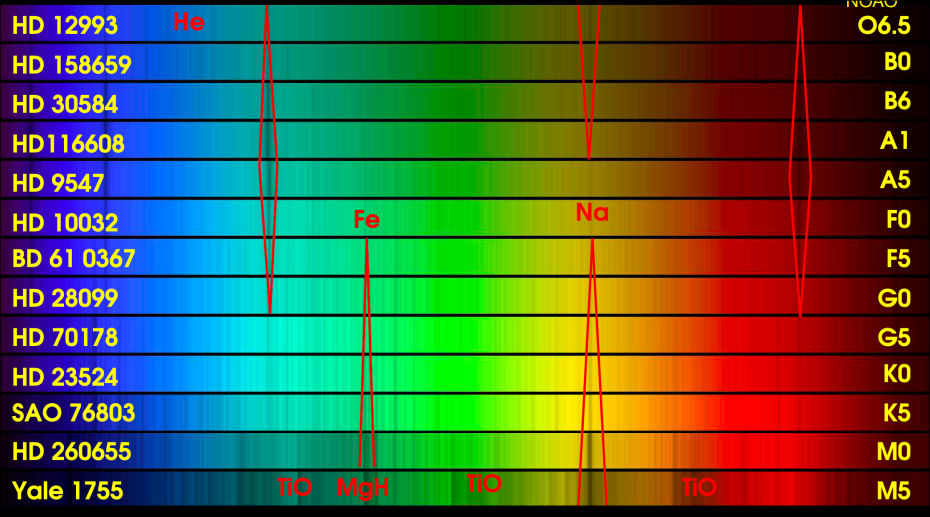
\includegraphics[width=0.6\linewidth]{screenshot_2024-01-19-192210.png}
\end{center}
Classes O - B - A - F - G - K - M ranging from 30 000 K "early type" to 3000 K "late type" (this has nothing to do with the actual age).
"Oh be a fine guy/girl kiss me" \footnote{idk as long as i get a good smooch.}
\subsection{Double stars}
50 $\%$ to 80 $\%$ of stars are in multi star systems.

Classification:  
\begin{itemize}
    \item  
    Apparent binaries are stars that just look like they are binaries because of line of sight. 
    \item 
    Visual binaries are stars that can visually be determined to be binaries.
    \item 
    Spectroscopic binaries are stars that can not be visually resolved into binaries.
\end{itemize}
Binaries often wobble. 
Their masses can be determined by Kelpers third law.
While the period can be measured the semimajor axis depends on the inclination and distance.
Velocity of orbit is 
\begin{align*}
    v_r = v sin i cos (wt)    
\end{align*}
This motion is visible through Doppler shift.
\begin{align*}
    \frac {\Delta \lambda}{\lambda} &= \frac {v_r}{c} = \frac {v}{c} sin i cos wt 
\end{align*}
\subsection{Mass-Luminosity Relation}
For M $<$ 0.42 $M_\odot$: 
\begin{align*}
    \frac {L}{L_\odot} &= 0.23 \frac {M}{M_\odot}^{2.3} 
\end{align*}
and for M $>$ 0.42 $M_\odot$: 
\begin{align*}
    \frac {L}{L_\odot} &= \frac {M}{M_\odot}^{4} 
\end{align*}
This leads to the conclusion that massive stars have much shorter lives.
\begin{center}
    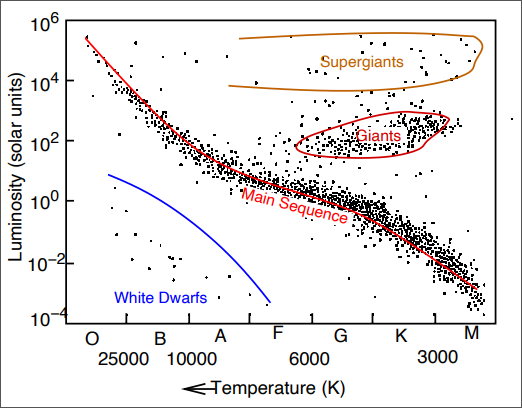
\includegraphics[width=0.6\linewidth]{screenshot_2024-01-19-194120.png}
\end{center}
Because of 
\begin{align*}
    L &= 4 \pi R^2  \rho T^4 
\end{align*}
cold and luminous stars are big (giants).

\subsection{Variable Stars}
Most stars show relatively constant luminosities, while some others show large changes from years to fractions of seconds in length.
Physically there are three main types of variable stars:
\begin{itemize}
    \item pulsating variables \\
        Here the shifts in luminosity coincide with shifts in the spectral lines.
        This is usually due to quick shifts in the atmospheres of stars. 
        The most important subtypes are: 
        \begin{itemize}
            \item Cepheids \\ 
                Pulsating supergiants \\ 
                link between period and absolute magnitude 
            \item RR Lyrae stars \\ 
                about to undergo helium burning\\ 
                very common in globular clusters \\ 
                The absolute magnitude is constant and known 
            \item Many other types exist too
        \end{itemize}
    \item eruptive variables \\  
        Here sudden outbursts go along with ejection of stellar material  
        The most important subtypes are: 
        \begin{itemize}
            \item UV Ceti stars \\ 
                red-main sequence stars \\ 
                variable brightness up to $6^m$ \\ 
                outbursts in corona or chromosphere (similar to solar flairs)
            \item R Coronae Borealis stars \\ 
                Supergiants of class F \\ 
                sudden loss of brightens and mass up to 10 mag and large loss of mass \\ 
                formed by formation of dust shells
            \item T Tauri and RW Aurigae stars\\ 
                young stars (pre-main sequence) of type G or later\\ 
                strong mass variations 
            \item cataclysmic type eg. supernovae 
        \end{itemize}
    \item eclipsing variables eg. variables  
\end{itemize}
\begin{center}
    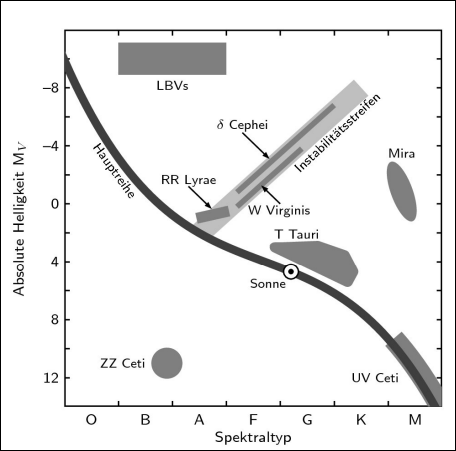
\includegraphics[width=0.6\linewidth]{screenshot_2024-01-21-173647.png}
\end{center}
This can be interpreted as stars staying in their position in the HRD for most of their lives.
The stars become variable during certain parts of their evolution during so called instability regions.
\subsection{The inner structure of stars}
The inner workings of stars are controlled by four factors: 
\begin{itemize}
\item Mass conservation \\
    Density stratification of a star is defined through mass conservation:
    \begin{align*}
        M(r) &= \int_0^r 4 \pi r^2 \rho (r) dr \\
    \end{align*}
        \text {and therefore:} 
    \begin{align*}
        \frac {dM}{dr} &= 4 \pi r^2 \rho (r)  
    \end{align*}
    \begin{center}
        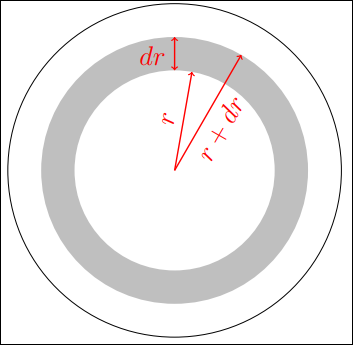
\includegraphics[width=0.3\linewidth]{screenshot_2024-01-21-174522.png}
    \end{center}
\item Movement conservation (Hydrostatic equilibrium) \\
    Pressure stratification of a star is defined through hydrostatic equilibrium:

        \text{Gravitational}\text{ force between M(r) and a slab of gas dAdr:} 
    \begin{align*}
        dF_g = - \frac {GM_r dm } {r^2} &= - \frac {GM_r \rho (r)} {r^2} dAdr \\
    \end{align*}
        \text{force due to pressure gradient:}
    \begin{align*}
        dF_P = dA(P(r+dr) - P(r)) &= dAdP \\
    \end{align*}
        \text{therefore:} 
    \begin{align*}
        \frac {dP}{dA} &= - \rho (r) \frac {GM}{r^2}
    \end{align*}
    \begin{center}
        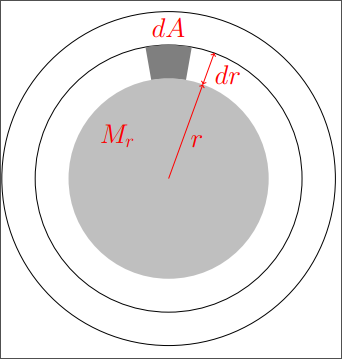
\includegraphics[width=0.3\linewidth]{screenshot_2024-01-21-174815.png}
    \end{center}
\item Energy conservation \\
    Temperature stratification of a star is defined through energy conservation and
energy transport: \\
let $\epsilon$ be the energy produced per time and mass 
\begin{align*}
    dL &= \epsilon dM_r = 4 \pi \rho (r) \epsilon dr \\ 
    \frac {dL} {dr} &= 4 \pi r^2 \rho (r) \epsilon
\end{align*}
    \begin{center}
        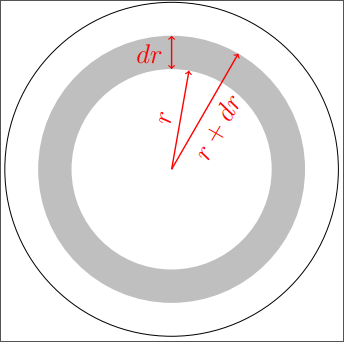
\includegraphics[width=0.3\linewidth]{screenshot_2024-01-21-180043.png}
    \end{center}
\item Energy transport \\
    in stars energy is mainly transported by radiation and convection. 
    In an optically thick medium a radiative process is usually diffusive.
    This leads to diffusion theory: 
    \begin{align*}
        \frac {dT} {dr} = - \frac {3} {4 a c} \frac {k(r) \rho (r)} {T^3} \frac {L(r)}{4 \pi r^2} 
    \end{align*}
    Convection cannot be describe self consistently so approximation: 
    \begin{align*}
        \frac {dT} {dr} = -(1 - \frac {1}{\gamma}) \frac T P \frac {dP}{dr}
    \end{align*}
    with $\gamma$ as the adiabatic index. 
    1 for an ideal gas, 5/3 for a degenerate gas and 4/3 for relativistic matter
\end{itemize}
To solve this a equation for P is needed. 
Due to high temperature generally a ideal gas law is followed: 
\begin{align*}
    P &= \frac {k_B}{\mu m_H} \rho T 
\end{align*}
with $\mu$ being the mean molecular weight and $m_H$ the mass of a hydrogen atom.

Due to very high pressures radiation pressure comes into the fold: 
\begin{align*}
    P_{rad} &= \frac 1 3 a T^4 
\end{align*}
with a being the radiation constant.

At very high densities quantum mechanical effects come into play: 

The Pauli exclusion principle: \\
For particles such as electrons (“Fermions”), at least one of their quantum numbers must be different.

These numbers are: 
\begin{itemize}
    \item position 
    \item momentum 
    \item angular momentum 
    \item spin
\end{itemize}
All of these are quantized. 
According to the Heisenberg-principle 6-d phase space is quantized: 
\begin{align*}
   \Delta p \time \Delta V \approx h^3 
\end{align*}
Therefore each "cell" in phase space can host two electrons (due to spin). 
This becomes a problem when the pressures get to high. 
Therefore in degenerate matter electrons have much higher energies. 
\begin{align*}
    \rightarrow P \propto \rho^{5/3} 
\end{align*}
Their velocities can become close to the speed of light and therefore be:
\begin{align*}
    \rightarrow P \propto \rho^{4/3} 
\end{align*}
The resulting equations for stars have to be solved numerically. 
The results are: 
\begin{itemize}
    \item Core temperatures of $>$ $10^7$ K. Bulk luminosity
released in the core. 
    \item Low-mass
stars have a radiative core and convective outer layers. The structure
of high-mass stars is reversed.
\end{itemize}
The resulting energy can be released by fusing light elements into heavy elements. 
This does however reach an end at iron.
\subsection{Nuclear fusion}
In general fusion of Helium into Hydrogen 
\begin{align*}
    4p \rightarrow \text{ }^4_2 He + E
\end{align*}
Energy released can be calculated by $E=mc^2$ 
and is about 25 MeV. 
In the fusion of hydrogen to helium, 0.7\% of the available rest mass energy is converted to energy.
The two main burning cycles are the proton proton chain and the CNO-Cycle
for reference see slides.
\section{Stellar evolution}
\subsection{Dynamical Timescale}
How long does it take for a star to collapse if pressure support against gravity is suddenly removed?
\begin{align*}
    t_{dyn} &= \frac {R} {v_{escape}} = \sqrt{\frac {R^3}{2GM}}
\end{align*}
For the sun its 1100 s.
\subsection{Kelvin-Helmholtz Time Scale}
Suppose nuclear reactions were suddenly switched off in star. How long does it
take to radiate away all its thermal energy?
\begin{align*}
t_{HK} &= \frac {GM^2}{RL} 
\end{align*}
In the case of the sun about $3 \cdot 10 ^7$ Years.
\subsection{Nuclear Time scale}
Assume constant burning rate. How long does it take for the star to exhaust its
supply of nuclear fuel?
\begin{align*}
    t_{nuc} &= \frac {E_{nuc} }{L} = \frac {qXM \cdot 6 \cdot 10^{18} erg/g}{L} = \frac M L \frac {M_\odot}{L_\odot} \cdot 7 \cdot 10^9 yr
\end{align*}
for the sun this is around $ 7 \cdot 10 ^9 $ years. \\
X: mass fraction of H initially present; q fraction of fuel that actually gets burned
composition of stellar material contains about 70\% of hydrogen; usually 10% of
this is burned in stellar evolution
\subsection{Stellar Birth}
Stars are born in "Giant molecular clusters".
These are large clouds with diameters of 5-100 pc containing lots of H,He, alcehol, ... . 
They are the coldest regions of the interstellar medium with 10-100K and have typical densities of thousands to Millions of particles.

Stars are born when these clouds collapse.
They collapse when gravitation is stronger than the thermal pressure. 
Collapse is possible when the radius r: 
\begin{align*}
    R > R_J &= \sqrt{\frac{15kT}{8 \pi Gm_p \rho}} 
\end{align*}
where $R_J$ is the Jeans radius.
The mass is then: 
\begin{align*}
    M_J &= \frac {4}{3} \pi R^3_J \rho 
\end{align*}
This mass is 50-100 solar masses typically. 
Star formation would generally be far to strong.

Luckily magnetic fields can explain the discrepancy.

During contraction gravitational energies get turned into thermal energies. 
During the initial low density and low opacity stages most of the heat gets transported via radiation on the dynamical timescale. 
Later on density and opacity increase leading to more radiative energy turned to heat. 
Due to higher temperature and pressure the contraction slows down and the protostar is formed.
At 1800 K $H_2$ starts dissociating and at 10000K H, He stars ionizing. 
This consumes energy leading to a temporarily speed up collapse.

At $10^5$K the gas is fully ionized and formed a plasma.
The star now reaches Hydrostatic equilibrium and evolves on the KH timescale.
Temperature being low and high opacity lead to loads of convective energy transport and therefore high brightness.
\begin{center}
    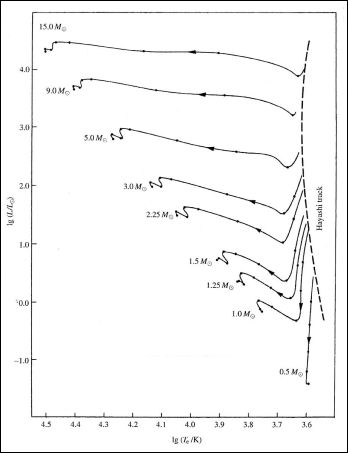
\includegraphics[width=0.5\linewidth]{screenshot_2024-01-21-194512.png}
\end{center}
\begin{itemize}
    \item at the beginning the cold star is on the far right
    \item As the surface heats up it moves to the upper right
    \item end of collapse: settles to point on the
Hayashi track (location of completely convective stars) corresponding to its mass
    \item evolution downwards on Hayashi track on KH timescale as radius decrees and L drops
    \item as nuclear energy generation becomes important the star becomes more and more radiative 
    \item the star then moves from the Hayashi track to the main sequence
\end{itemize}
(EGGS in presentation)

\section{The expansion of the universe}
Galileo discovered that the universe is made up of stars.
Messier found nebula. 
Bessel first determined stellar parallax. 

The great debate: 
Is Andromeda part of our galaxy.
Solved by Edwin Hubble detecting Cepheid's in Andromeda allowing for distance measurements.
\subsection{Structure of the milky way}
\begin{center}
    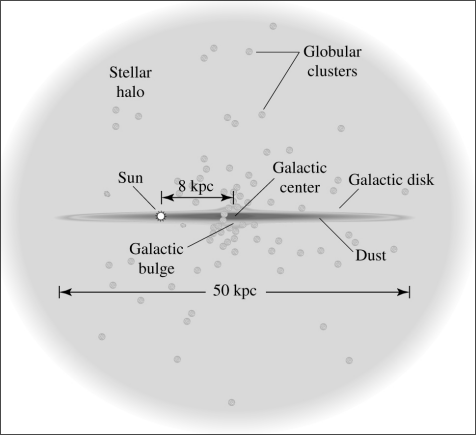
\includegraphics[width=0.5\linewidth]{screenshot_2024-01-23-105305.png}
\end{center}
Components: 
\begin{itemize}
    \item Rotating disk filled with young and old stars, open star clusters and gas \& dust 
    \item non rotating galactic halo filled with old stars, globular clusters and no dust and gas 
    \item galactic bulged with rigid rotating bars
\end{itemize}
\subsection{Expansion} \label{sec:Expansion}
velocity is defined by: 
\begin{align*}
    \frac v c &= z = \frac {\Delta \lambda} {\lambda} 
\end{align*}
Distance of galaxies measured by Edwin Hubble, got the following relation:
\begin{align*}
    v(r) &= H_0 t 
\end{align*}
Currently different detection methods give different answers. 
Galaxies are at distances of megaparsec to larger.
We are not the center of the universe, the expansion is a isomorphism.

\subsection{Distance determination}
The nonage of distances is required to determine other things like Luminosity or mass or Size. 
There does however only exist one direct method:  Trigonometric parallax. 
Most other methods are based on "standard candles" i.e. objects with know brightness. 
For example:
\begin{itemize}
    \item Main sequence fitting
    \item Variable stars: RR Lyrae and Cepheids
    \item type 1a supernovae 
    \item Tully-fisher spiral galaxies 
    \item $D_n-\rho$ for ellipticals 
    \item Brightest galaxies in a cluster
\end{itemize}
We might also use Hubble's law.
These methods are calibrated using the previous steps on the distance ladder.

\subsection{Standard candles}
See also \ref{Distance Modulus}
Standard candles are defined to be objects for which their absolute
magnitude is known.

Therefore we have two requirements:
\begin{itemize}
    \item the physics of a candle are well known 
    \item the absolute magnitude of a standard candle can be calibrated e.g. we can measure the distance via other means.
\end{itemize}
To determine distance to astronomical object:
\begin{itemize}
    \item find standard candle near object 
    \item measure the m
    \item determine m - M, M is known from candle 
    \item compute the distance
\end{itemize}
\subsection{main sequence fitting}
A HRD can be shifted till the main sequence aligns with the theory.
From this we can determine the distance modulus.
This only works up to 7 kPC. 

\begin{center}
    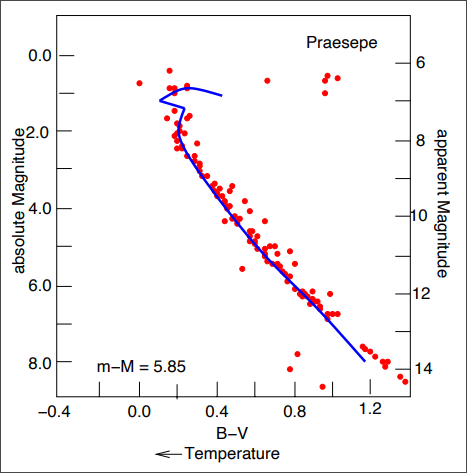
\includegraphics[width=0.5\linewidth]{screenshot_2024-01-23-112801.png}
\end{center}
\subsection{variable stars}
Certain regions of the HRD are unstable and therefore produce variable stars:
\begin{center}
    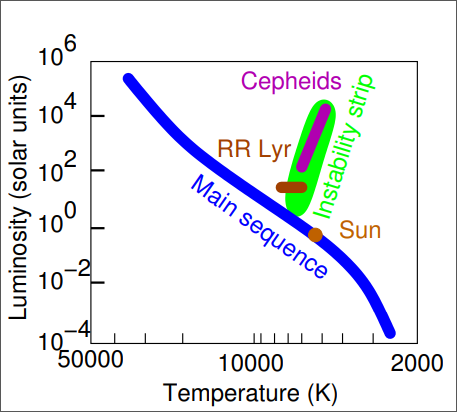
\includegraphics[width=0.5\linewidth]{screenshot_2024-01-23-113048.png}
\end{center}
The most important variable stars are: 
\begin{itemize}
    \item RR Lyrae, I \\ 
        These are mainly found in globular clusters due to lower metalicyty of the clusters.
        Period of 0.2 to 1 days, mainly changes in temperature\\ 
        Absolute magnitude of RR Lyare gap between 0.6-0.8 mag ~ 50 $L_\odot$ \\
        works to around d = 50 kPC so only for local group
    \item Cepheids \\ 
        Luminous stars (L ~ 1000 $L_\odot$) with large changes in luminosity with a period of 2-150d
\begin{center}
    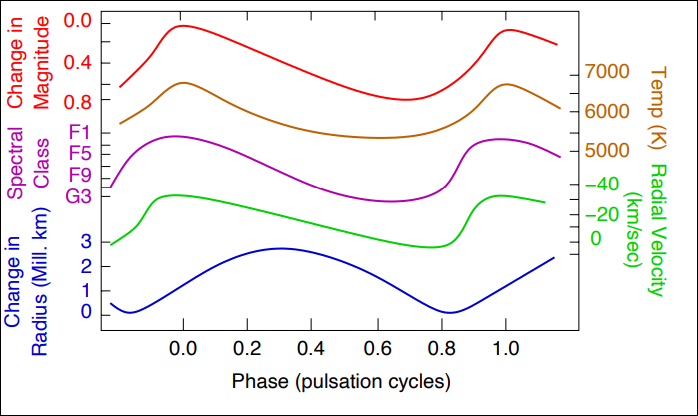
\includegraphics[width=0.5\linewidth]{screenshot_2024-01-23-113927.png}
\end{center}
    Period to luminosity relation discovered by Henrietta Leavitt: 
     \begin{align*}
       M = -2.76 log P - 1.4 
     \end{align*}
     with P in days.
\end{itemize}
Other standard candles include: 
\begin{itemize}
    \item Supernovae 
\begin{center}
    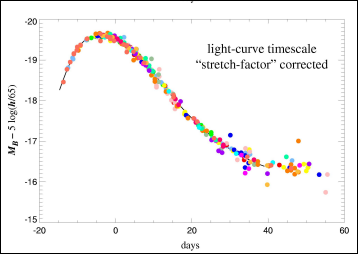
\includegraphics[width=0.5\linewidth]{screenshot_2024-01-23-114223.png}
\end{center}
After corrections of systematic affects and time dilation all type 1a supernovae have the same light curves.
They occur when white dwarf are pushed over the Chandrasekhar limit of 1.4 Solar masses.
They have a very characteristic light curve with a fast rise, rapid fall and exponential decay with a halftime of 60 days.
Calibration: SNe Ia in nearby galaxies where Cepheid distances known
Observable to up to 1GPc or grater.
\end{itemize}

\subsection{The main sequence}
Once star has collapsed and nuclear fusion has started, i.e., after a few Million years: zero age main sequence
The main sequence is the result of most stars burning Hydrogen into helium for the longest part of their existence.
The time spend on the main sequence depends on the stellar mass and is shorter for larger stars.
\begin{center}
    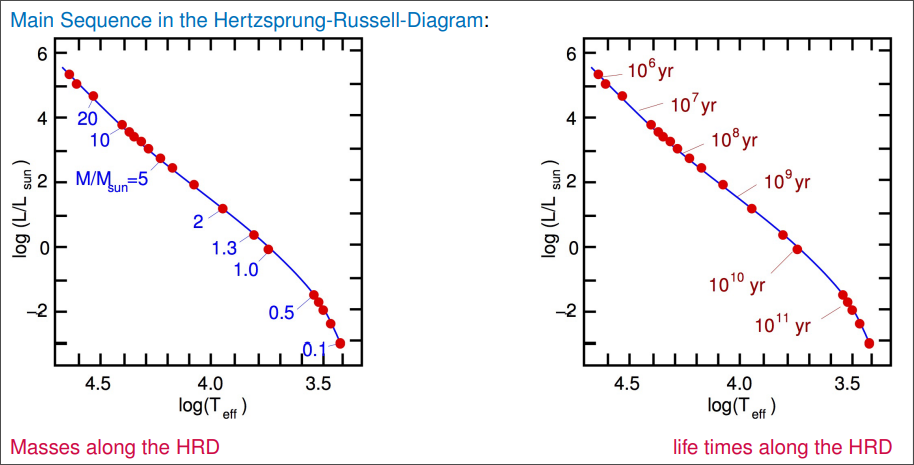
\includegraphics[width=0.5\linewidth]{screenshot_2024-01-23-115246.png}
\end{center}
\begin{center}
    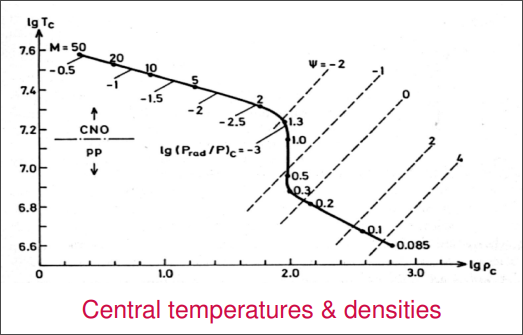
\includegraphics[width=0.5\linewidth]{screenshot_2024-01-23-115334.png}
\end{center}
Strong change in stellar structure observed at 1 Stellar mass. 

$< 0.5 M_\odot$ low temperature and high density. \\
$> 1.3 M_\odot$ high temperature and low density. \\
Low mass stars burn H in pp-chains and high mass stars burn H in the CNO cycle.
The upper main sequence stars are: 
\begin{itemize}
    \item high central temperature leading to the CNO cycle.
    \item high temperature sensitivity
    \item large outward energy flux leading to a large temperature gradient 
    \item convective core 
    \item no nuclear reactions outside of core, leading to it being held up by radiative equilibrium 
\end{itemize}
$\rightarrow$ Upper main sequence stars have a convective core and radiative shell. 
The lower main sequence stars are: 
\begin{itemize}
    \item lower central temperature leading to the PP-chain.
    \item lower temperature sensitivity leading to burning in a larger area
    \item radiative core 
    \item no mixing in core leading to He abundance increasing outwardly
    \item low temperature in outer shell leading to high opacity and therefore to convection
\end{itemize}
$\rightarrow$ lower main sequence stars have a radiative core and convective shell. 

The lower the temperature the further the convective shell reaches into the core. 
This leads to stars with low core temperature becoming fully convective and unstable (i.e. they might only exist as brown dwarfs)
\begin{center}
    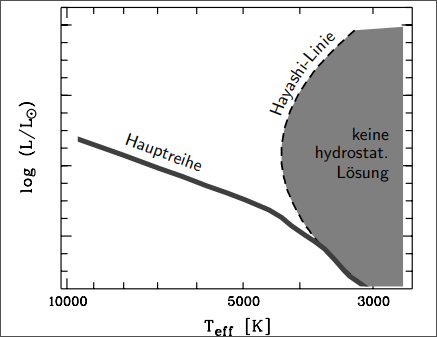
\includegraphics[width=0.5\linewidth]{screenshot_2024-01-23-122838.png}
\end{center}
\subsection{Stellar evolution on the HRD}
The processes that happen when a star burn all its helium depend on its mass: 

Stars with masses above 2.5 solar masses: 
\begin{center}
    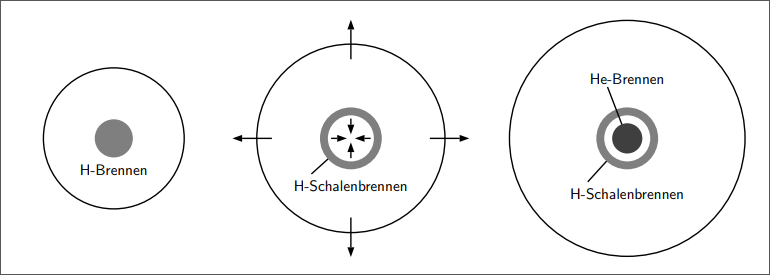
\includegraphics[width=0.5\linewidth]{screenshot_2024-01-23-123306.png}
\end{center}
Hydrogen burning ends. This leads to the radiation pressure decreasing. 
This then leads the He core to contract and heat up. 
This conversion of potential into thermal energy leads the H envelope to expand quickly. 
The H shell then starts burning while the He core contracts further, heats up and gains mass. 
At temperatures larger than $10^8$ K He burning stars. 
This looks like the following on the HRD (high mass stars): 
\begin{center}
    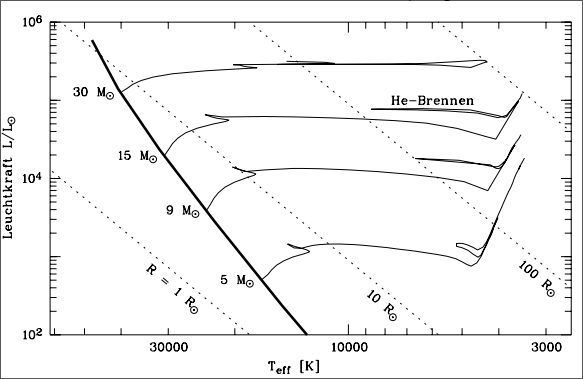
\includegraphics[width=0.5\linewidth]{screenshot_2024-01-23-123659.png}
\end{center}
where The fast movement to the right is explained by the expansion (on KH timescale) followed by a slow evolution on the red giant regime during He burning (nuc. timescale)
By the point where the stars in the HRD of a galaxy branch off we can tell their age. 

For smaller stars a somewhat similar process takes place: \\
He core contracts on Kh timescale leading to the conversion of potential to thermal energy leading to the H envelope expanding.
The star then moves quickly to the right on the HRD. 
However as the core contracts more and more the matter becomes degenerate at some point leading to a stop in temperature increase as we dont have a ideal law anymore. 
This means that He burning cannot start right away. 
The contraction then stops due to degeneracy pressure. 
Due to H burning in the shell the mass of the He core still increases. 
The luminosity then strongly depends on the mass of the He core.
Finally the star enters the read giant phase. 

Once the degenerate core reaches 0.26 Solar masses at $10^8$ K the triple alpha process stars. 
The as P $\neq$ P (T) in degenerate matter the core cannot cool through expansion. 
The increasing temperature accelerates the burning rate leading to a runaway process that ends in a helium flash. (Explosive He burning)
After this the heat up in the envelope ends the degenerate state leading the star to start He burning in the core and Helium burning in the shell. 
The core then expands again leading to less efficient burning in the shell. 
The luminosity then decreases and the star ends up on the horizontal branch. 
\begin{center}
    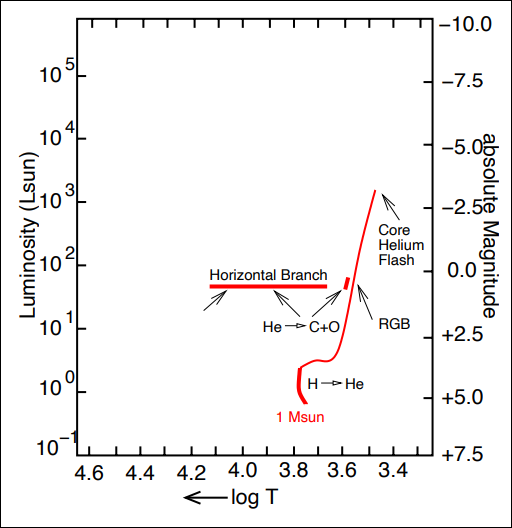
\includegraphics[width=0.5\linewidth]{screenshot_2024-01-23-125357.png}
\end{center}
After all the He is burned up the C/O core starts to contract. 
As the envelope expands the luminosity rises along the Asymptotic giant branch. 
Instability and strong stellar wind lead to the star loosing its outer layers (50\% of mass). 
\begin{center}
    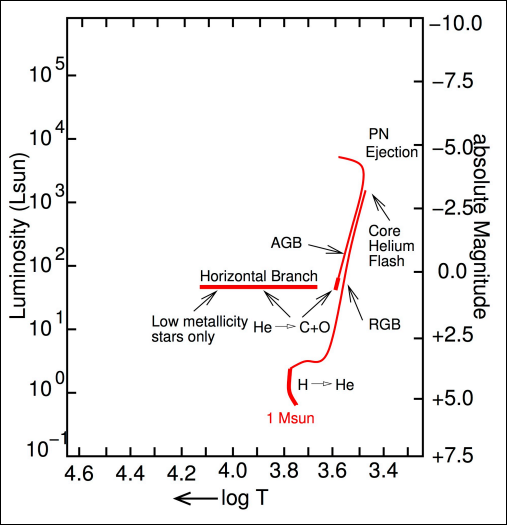
\includegraphics[width=0.5\linewidth]{screenshot_2024-01-23-125721.png}
\end{center}
\subsection{Planetary nebulae}
Fore both Massive and lighter stars stellar envelopes form around C/O core. 
The mass of the core depends on the initial mass and is around 0.6-0.85 Solar masses.
As the star begins to cool it forms a white dwarf. 
\begin{center}
    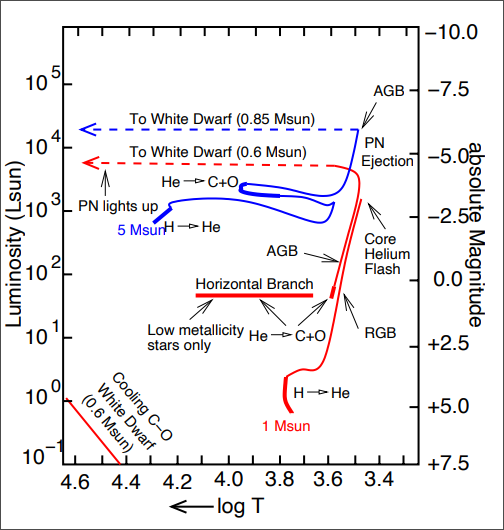
\includegraphics[width=0.5\linewidth]{screenshot_2024-01-23-125950.png}
\end{center}
The structure of a white dwarf can be determined form Hydrostatic equilibrium and mass conservation alone, as P is independent of T in degenerate and relativistic gasses. 
We now have a mass radium relation of: $T \propto M^{-1/3} $ for non relativistic gases and $T \propto M^{-\infty} $ for relativistic gasses.
The Chandrasekhar limit tells us that the mass must be less than 1.4 solar masses or the star will collapse as no hydrostatic equilibrium is possible.

The remaining white dwarf are stabilized by the pressure of the degenerate electron gas. 
They cool down slowly into a diamond like crystal stricter.


For super massive stars the process is a bit different: \\
For stars with a mass of more than 8 Solar masses: \\ 
After the He burning stops the nuclear time scale becomes short compare to the thermal time scale of the outer layers.\\
Whit masses of around 10 Solar masses carbon and oxygen burning becomes possible. (in a oxygan flash)
For even more massive stars no explosive states take place leading to a bunch of shells burning different elements: 
\begin{center}
    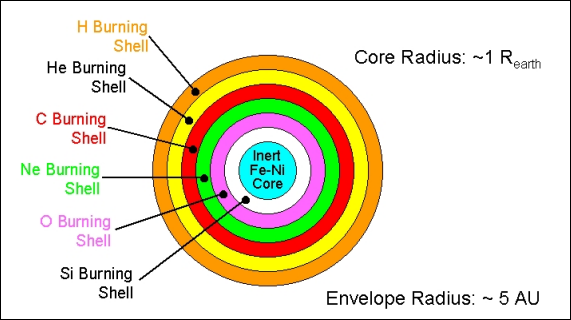
\includegraphics[width=0.5\linewidth]{screenshot_2024-01-23-131219.png}
\end{center}
The ash of the previous stage becomes the flue for the next.
This process stops at Fe as it has one of the most tightly bound nuclei. 
As the core exceeds a density of $3 \cdot 10^{12} gcm^{-3}$: 
\begin{itemize}
    \item $e^- + p \rightarrow n + v_e  $ leading to a decrease in electron abundance in the core witch leads to a drop in pressure. 
    \item The Chandrasekhar mass than falls below the mass of the iron core leading to a core collapse. 
\end{itemize}
This core collapse takes place on the dynamic timescale with around 1 ms time.
The collapse leads to a further increase in pressure. 
As this pressure reaches $10^{14} gcm^{-3}$ the nuclear force leads to a sudden stiffening in the equations of state and outer matter to bounce back as a shock wave propagates outwards.
This releases more than $10^45 J$ and loads of notions as outer layers expand at $10^4 kms^{-1}$ and the star exploding in a core collapse supernovae.
The collapsing core either stabilizes as a neutron star or (depending on
mass and structure of the progenitor star) collapses to a black hole.
\section{Supernovae}
Classification:
\begin{itemize}
    \item No H lines $\rightarrow$ type 1, 1a when silicone lines and  1b,c when No si lines. 
    \item H liens $\rightarrow$ type 2
\end{itemize}
The different emission lines suggest different compositions of the outer shells of stars. 
The light curves of type 1 are all very similar as opposed to the light curves of type two, which scatter more. 
\begin{center}
    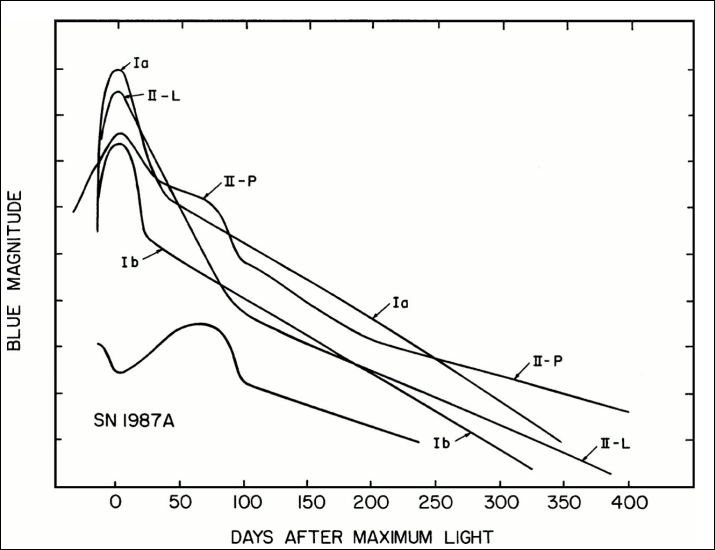
\includegraphics[width=0.5\linewidth]{screenshot_2024-01-24-104355.png}
\end{center}
Type 2-L resemble type 1, while type 2-p have a more constant brightness after their peak withing a 1 mag range for a while.

Around half of all supernovae are type 2, while type 1a is around a quarter and 2b a fifth.

The observed energy is around $10^{51}$ erg leading to gravitational binding energy and nuclear energy as the source. 

Types 2, 1b and 1c generally come from star forming regions ins the spirals of galaxies.
This leads to the conclusion that their progenitor's are massive stars and that they are powered by the gravitational energy release under formation of a neutron star or black hole during core collapse. 

Type 1a is probably caused by thermonuclear explosion of carbon-oxygen white dwarfs as they come form regions of space with older, lighter stars. 

This leads to the progenitor problem, as the progenitor system generally cant be observed. 
However white dwarfs need a companion to reach the energy's required to undergo 1a. 
Therefore there are two main models:
\begin{itemize}
    \item "Single-degenerate system", systems in which the WD accretes matter from another star.
    \item “Double-degenerate system”, systems in which two WD merge. 
\end{itemize}
\begin{center}
    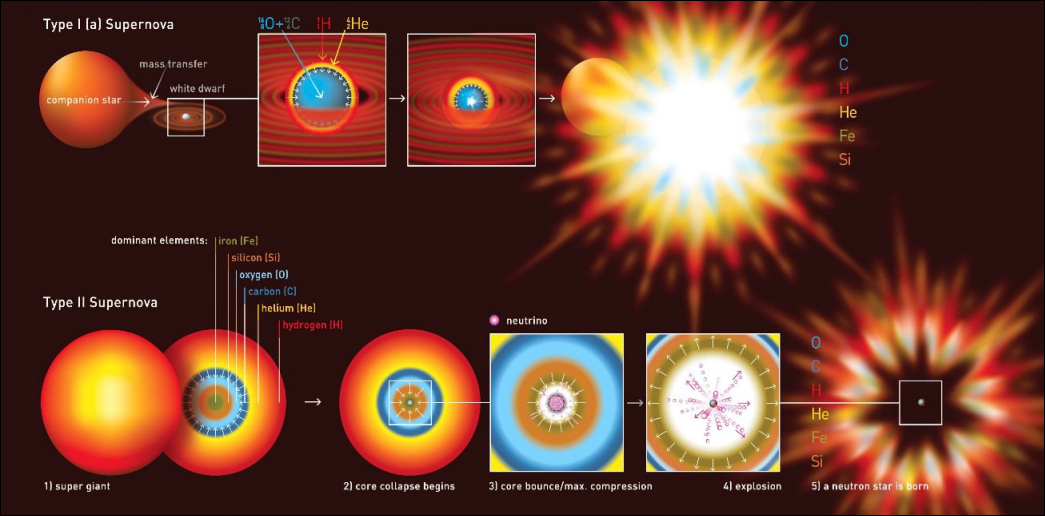
\includegraphics[width=0.9\linewidth]{screenshot_2024-01-24-105703.png}
\end{center}
during SN1987a the progenitor star was able to be observed. 
It was a massive star in the Large Magellanic could.
This supports the core collapse model. (for more see slides)

\subsection{End stages of stars}
Generally stars end up as compact objects. 
\begin{itemize}
    \item white dwarf: \\ 
    $\rho$ of $10^5$ to $10^6$ $gcm^{-3}$, R ~ $R_\mathTerra$, In equilibrium between gravitation and degenerate pressure of electrons
    M $<$ 1.44 $M_\mathSun$ (Chandrasekhar-Limit)
\item Neutron star:  \\ 
    $\rho$ of $10^{13}$ to $10^{16}$ $gcm^{-3}$, R ~ 10 km, In equilibrium between strong interactions and degenerate pressure of neutrons
   1.44 $<$ M $<$ 3 $M_\mathSun$ (Oppenheimer-Volkoff Limit)
\item Black hole: \\ 
    3 $M_\mathSun$$<$ M, No stable state  is known, event horizon at $3 \frac M M_\mathSun$ km
\end{itemize}
Therefore compact objects with more than three solar masses are black holes.

\subsection{Neutron Stars}
During collapse the angular momentum is conserved. 
\begin{align*}
    J &= I \omega \\ 
    I &= \frac 2 5 MR^2
\end{align*}
By conservation of angular momentum we get: 
\begin{align*}
    \omega_{NS} &= \frac {M_{before}}{M_{after}} \frac {R_{before}}{R_{after}}^2  
\end{align*}
Therefore Neutron stars must rotate quickly. 

Pulsars are Neutron stars that pulse on the order of Milliseconds to seconds. 
This is called the lighthouse effect and is caused by the pulsars synchrotron beam quickly passing over the earth. 
This has a period of
\begin{align*}
    P &= \frac {2 \pi R}{v_rot} 
\end{align*}
Due to the short period time and the pulsar having to rotate slower then the speed of light the radius has to be small. (bellow 50km)
Magnetic flux $\Phi = BR^2$ is also conserved. 
Therefore we get:
\begin{align*}
    B_{NS} &= \frac {R_{before}} {R_{NS}}^2 B_{before} 
\end{align*}
This leads strong magnetic fields. 
Typically $10^6$ to $10^8$ T. 

This leads to the conclusion that pulsars are quickly rotating neutron stars with strong magnetic fields that emit through synchrotron radiation.

\subsection{Black hole X-ray binaries}
Matter flows from a companion star via Lagrange point L1 onto compact object.
This leads to the forming of a accretion disk and loads of X-ray and $\gamma$ ray radiation.
\begin{center}
    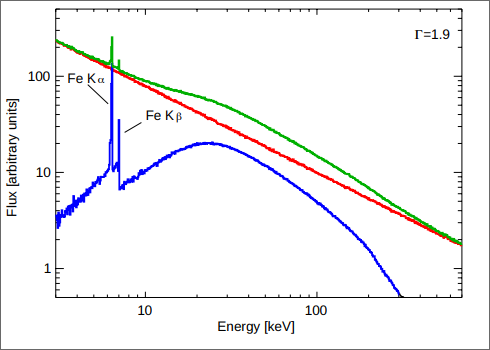
\includegraphics[width=0.5\linewidth]{screenshot_2024-01-24-113302.png}
\end{center}
green: Hard X-rays, Thompson scattering in accretion disk leads to Compton Reflection Hump
red: Comptonisation of soft X-rays in a hot plasma (T ~ $10^8$ K): power-law spectrum.
blue: Photon absorption of Hard X-Rays in the disk leads to Fe, K$\alpha$ lines. 
The Fe, K$\alpha$ spectrum is influenced by:
\begin{itemize}
    \item grav. Red shift
    \item rel. space curvature 
    \item rel. Doppler shift
    \item disk emission profile
    \item spin of the black hole
\end{itemize}
Relativistic broad iron
lines are observed in
many black-hole systems

The gravitational merger of black holes has been observed.
As expected no light emissions are produced. 

\section{Galaxies}
\begin{center}
    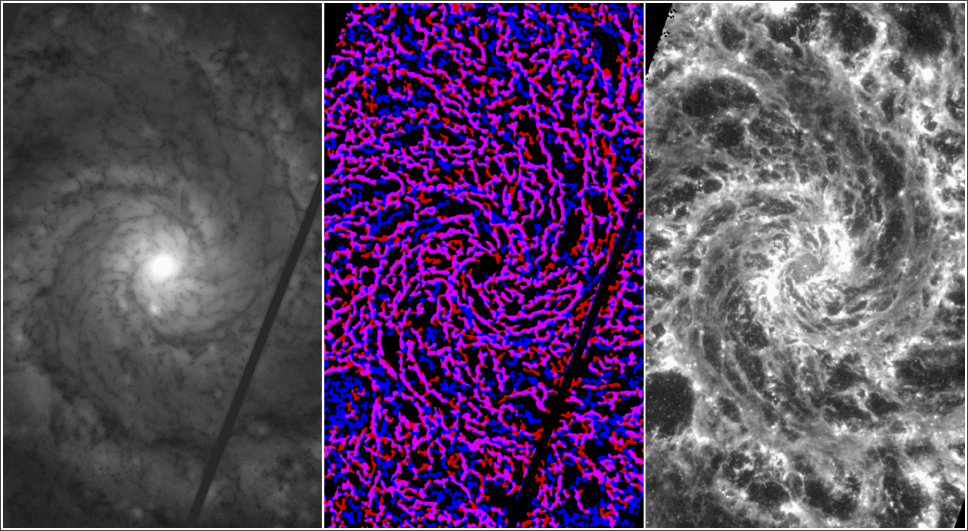
\includegraphics[width=1\linewidth]{screenshot_2024-01-24-120045.png}
\end{center}
Left: optical, middle dust filament network and right IR emissions

Bubbles in the ISM driven by feedback from young stars

\subsection{Observational problems}

\begin{itemize}
   \item Diameter: \\ 
       The edge of a galaxy is not well defined as the intensity falls strongly from center
   \item Small Galaxies cannot be distinguished
from stars
\item • Low surface brightness galaxies cannot be
seen against sky background
\end{itemize}
\subsection{The Hubble classification}
Classes are based on shapes of galaxies.
\begin{center}
    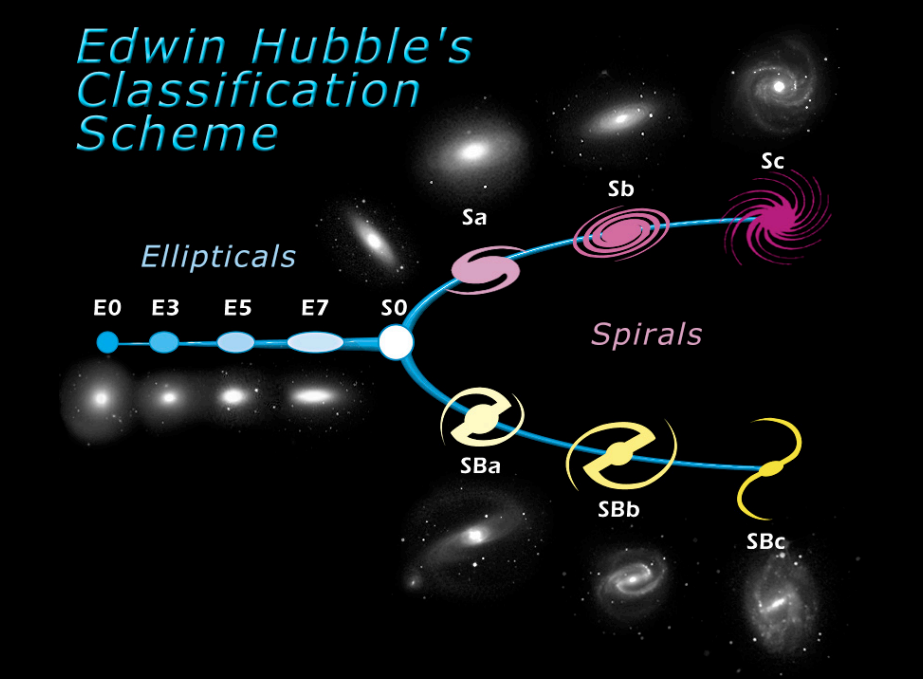
\includegraphics[width=0.8\linewidth]{screenshot_2024-01-24-120628.png}
\end{center}
"early types" are ellipticals while "late types are spirals"
Note: This is not a evolutionary series. 
The only type not present in the scheme are the cD galaxies which are the larges in a cluster. 
\subsubsection{Elipticals}
The early types are defined by: 
\begin{align*}
    x = 10 \frac {(1-b)}{a}
\end{align*}
This then is converted into a integer.
We however cant distinguish between the types as they depend on the angle.
There are three main types of ellipticals:
\begin{itemize}
    \item Luminous giant ellipticals: L $>$ $2 \cdot 10^{10} L_\mathSun$
    \item midsized ellipticals: $3 \cdot 10^9 <$ L $<$ $2 \cdot 10^{10} L_\mathSun$
    \item dwarf ellipticals: L $<$ $3 \cdot 10^9 L_\mathSun$
\end{itemize}
At lower luminosities we can also distinguish between:
\begin{itemize}
    \item Compact Ellipticals cE 
    \item Dwarf Ellipticals (dE): lower surface brightness and metallicity than cE
    \item Blue compact dwarf galaxies (BCD): unusually blue and an appreciable
amount of gas
\item Dwarf Spheroidals (dSph): very faint and difficult to find
\end{itemize}
Radial brightness distribution in ellipticals is
given by de Vaucouleurs’ law:
\begin{align*}
    log (\frac {I(R)}{I_e})  = - 3.3307 (\frac {R}{R_e}^{0.25}-1)
\end{align*}
Where $R_e$ is the radius that contains half of the luminosity.
\subsubsection{Spirals}
Elliptical bulge with spiral arms, type depending on the opening angle of spiral arm (and dominance of the bulge)

Sa: 10 deg, "c: 20 deg

They are bluer than ellipticals.

Mass content of about $10^{11} M_\mathSun$ with $\frac M L $ = 20.

The gas content of the galaxies increases from 1 \% at Sa to 8 \%  a Sc.

The spiral arms are most likely caused by density waves.

The radial intensity of the Bulge also follows the de Vaucouleurs' law. 
The radial intensity of the spiral is given by: 
\begin{align*}
    I(R) &= I_0 - \frac {R}{R_0} 
\end{align*}
with $R_0$ the thickness of the spiral. 
Barred galaxies are significantly similar.

S0 galaxies are luminous and red, while Sc and later are fainter and bluer.

\subsubsection{Irregular Galaxies}
\begin{itemize}
    \item Irr I: \\ 
        No symmetry or spiral arms, bright knots of O- and Btype stars, very blue (B - V ~ 0.5), high dust content around 16 \% large range of masses from $10^6-10^{10}$ solar masses
    \item Irr II: \\
        asymmetrical and “abnormal” basically all other objects. 
\end{itemize}
\subsubsection{Spectra}
The spectra of galaxies are the sum of all the constituent spectra.
\begin{itemize}
    \item S0: no young hot stars $\rightarrow$ “red”
spectrum; mainly absorption
lines from cool K stars (similar to
ellipticals) 
\item Sc: mainly blue and UV emission, i.e., hot and young stars;
emission lines from photoionized
emission nebulae
\end{itemize}
Spectrum of a stellar population at
age t can be determined via Population Synthesis.
\begin{itemize}
    \item Sensitive to star-formation history
    \item Comparison with observed spectra:
Ellipticals and S0 are dominated by
old stars
\item Little evolution after ~ 4 Billion
years.
\end{itemize}
\begin{center}
    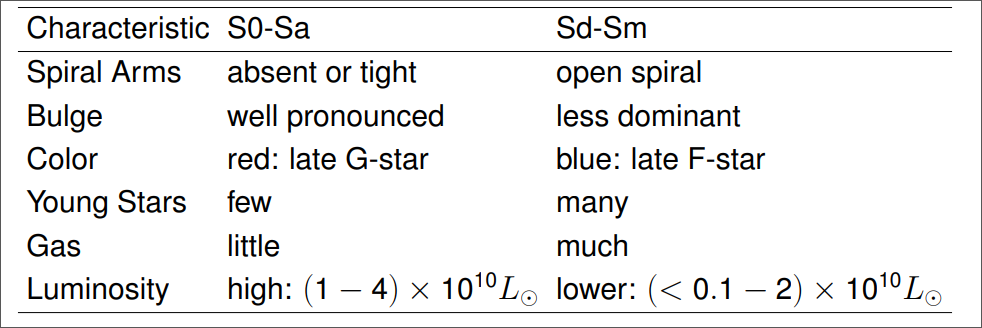
\includegraphics[width=0.8\linewidth]{screenshot_2024-01-24-123415.png}
\end{center}
\subsection{Dynamics}
The distribution of molecular and ionized hydrogen in a spiral galaxy
does more or less trace the star light distribution: Neutral H I has wider
distribution

 \paragraph{Hyperfine transitions}
 The base state of atoms is parallel (F=1), though metastable. 
 The transition to an antiparallel (F=0) state is possible but quantummechanically forbidden. 
 In the laboratory no transitions are observed as the F=1 state is depopulated by collisions. 
 Due to extremely low energies in the ISM no collisions happen and therefore the transition from F=1 to F=0 is possible.

 As our observations trace through multiple clouds of dust at differing rotations and different Doppler shifts the spectrum will look like: 
\begin{center}
    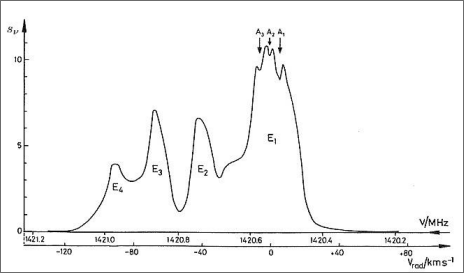
\includegraphics[width=0.8\linewidth]{screenshot_2024-01-26-124045.png}
\end{center}
A survey for the universe will look like:
\begin{center}
    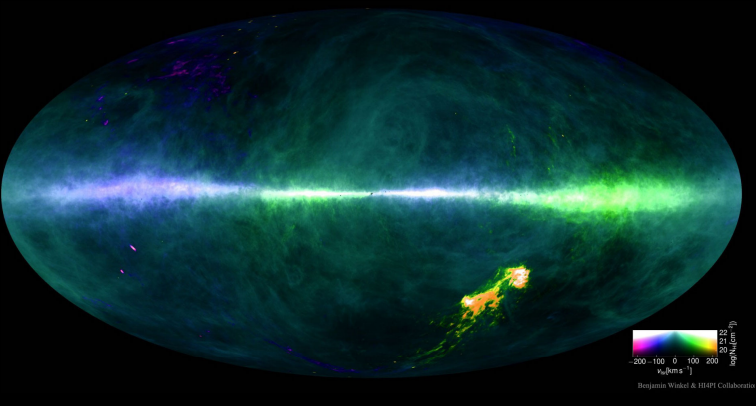
\includegraphics[width=0.8\linewidth]{screenshot_2024-01-26-124214.png}
\end{center}
The gas will generally extend to twice the optical radius of a galaxy.

Due to the movement of the stars in a galaxy we can observe different Doppler shifts and therefore calculate the rotational velocity of a point in a galaxy.
\begin{align*}
\frac {\Delta \lambda}{\lambda} &= \frac {v_r} c = \frac v c sin i
\end{align*}
This yields values of around 100 km$s^{-1}$ for spiral galaxies.
The only problem is that the rotational curves (i.e. The velocity towards the outer edge of galaxies) is fairly flat.
As:
\begin{align*}
    \frac {GM (< r) } r &= \frac {v^2_{rot}(r)} r \\  
    M (< r) &= \frac {v^2_{rot}(r)} G
\end{align*}
would imply the M($<$r) $\propto$ r.

Observations of the emitted light do however indicate that this isn't the case. 
Therefore we invoke dark matter: 
\begin{align*}
    M_{dark}(r) &= \frac M G (v^2 (r) - v_{lum}^2(r)) 
\end{align*}
where $v_{lum}$ is the expected velocity from the light distribution.

Observationally we can tell that the relationship between mass and luminosity is fairly constant at M/L ~ 10. (more precisely the 21 cm H line.)
This so called Tully-Fisher relationship can be used as a distance indicator. 
\begin{align*}
    V = - a log \left ( \frac {W_{20}}{sin i} \right ) - b
\end{align*}
where $W_{20}$ is : 20\% line width (km s-1
; typ. W20 ~ 300 km s-1
), i incl. angle, V abs. magnitude.
\subsection{Spiral patterns}
spiral arms can generally be described by: 
\begin{align*}
   cos (m(f(R,t) + \phi ))  = 1
\end{align*}
With R and $\phi$ being the coordinates along the galactic center m the number of arms and f the function that describes the winding. 
The opening angle is:
\begin{align*}
    cot i = \frac 1 {tan i} = |R \frac {\delta \phi} {\delta R}| =  |R \frac {\delta f} {\delta R}|
\end{align*}
For Sa i = 5 deg and for Sc i is between 10 and 30 deg.
There are two main types of spiral galaxies, 1. Grand design spirals and 2. Flocculant spirals.
There are different physical mechanisms at work in both. 
\begin{center}
    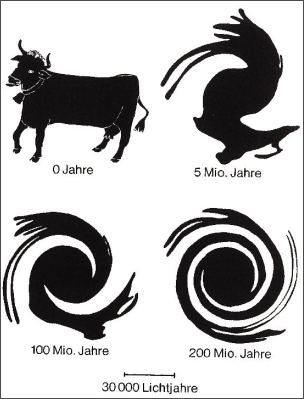
\includegraphics[width=0.3\linewidth]{screenshot_2024-01-26-135659.png}
\end{center}
Differential Rotation will wind up any instal radial structures and produce temporal spiral appearance on the disk. 
These so called stochastic spirals form very quickly.
The grand design spirals are formed by The density wave there:
The density wave theory of spiral structure explains assumes the growth
of such spiral patterns due to gravitational attraction of stars and gas
clouds at different radii and with different velocities. The pattern can rotate with a single pattern speed.
\begin{center}
    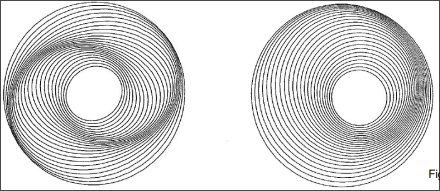
\includegraphics[width=0.6\linewidth]{screenshot_2024-01-26-140627.png}
\end{center}
Density-wave theory explains star-formation concentration towards spiral arms!
This is because compression of gas in the spiral arms. 

The bars observed in about half of all galaxies differ from the spiral arms. 
While they do have the same thickness they are browner than the spirals.
It is also apparent that the bars are rigid rotators. 
The bars do however appear to coronate with the spirals and are a likely cause of density waves. 

Simulations reveal:  \\
Stellar orbits close on themselves in corotating elliptical frames $\rightarrow$ Old enough populations are
distributed into elongated shapes
\begin{center}
    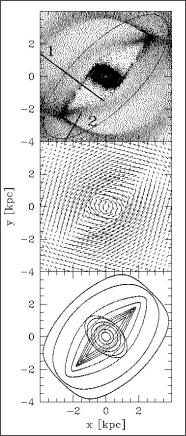
\includegraphics[width=0.3\linewidth]{screenshot_2024-01-26-141350.png}
\end{center}
Velocity gradients along the orbits cause shocks: 
\begin{itemize}
    \item Gas and dust are compressed
    \item Dust lanes along the bar major axis
    \item Energy dissipation leads to angular momentum transport
    \item Gas inflow towards galactic center
\end{itemize}
\subsection{Dynamics of elliptical galaxies}
Ellipticals show no (or
very little) ordered
rotation.
They also show a large velocity dispersion. 

A relation ship between velocity dispersion and brightness can be determined: 
\begin{align*}
    L &= \rho_c^4 
\end{align*}
Ellipticals do not rotate. 
However we are still able to estimate their masses unsung the viral theorem. 
\begin{align*}
    <E_{kin}> &= - \frac 1 2 <E_{pot}> 
\end{align*}
for ellipticals:
\begin{align*}
    M_G<v^2> &= G \int_0^{R_G} \frac {M(R)dM(R)} R = a \frac {GM^2_G}{R_G} 
\end{align*}
where for a homogeneous sphere a = $\frac 3 5$ and therefore:
\begin{align*}
    <v^2> = \rho^2  = a \frac{GM_G}{R_G} 
\end{align*}
Measurements show that the kinimetical mass in elliptical galaxies is significantly larger than the luminous mass.
Therefore dark matter must also be present in ellipticals. 
\subsection{MACHOS}
(Massive Compact Halo Objects): White dwarfs in the galaxy’s halo
This would explain the lack of visibility of Dark matter as white dwarfs aren't all that luminous. 
They are however detectable using micro lensing towards LMC and SMC. 
There are however factors that contradict this. 
Firstly the gravitational lensing has also been observed in normal stars in MW.
Secondly this would require a much larger formation rate. 
\subsection{Nonbaryonic matter}
This matter would have to interact with gravity but have no other or very few interactions with other matter. 

The first option for this would be non zero mass neutrinos. They do exist however only with very low masses.
They would have to be relativistic which dost fit current galaxy formation models.

A second option would be Axions (m$c^2$ ~ $10^{-5}-10^-{2}$eV) and WIMPS (weakly interacting massive
particles, GeV)
They would also help in cosmology, however we havent seen any sings of their existence. 
\subsection{Active galactic Nuclei}
\begin{center}
    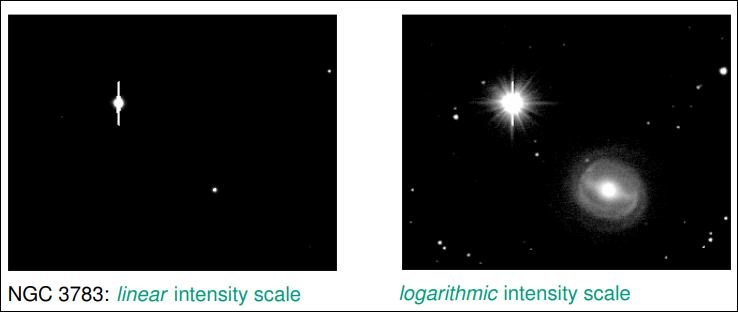
\includegraphics[width=0.8\linewidth]{screenshot_2024-01-26-145556.png}
\end{center}
We are able to see some massive y bright point like objects.
These are caused by so called active galactic nuclei. These are supper massive black holes ($10^6-10^8 M_\mathSun$) that acret around 1-2 $M_\mathSun$ per year.
Their light is around $10^{10} L_\mathSun$ so about as bright as a galaxy.

Observationally they are: \\
AGN are nuclei of galaxies, which show energetic phenomena that cannot be clearly and directly attributed to stars.
they show: 
\begin{itemize}
    \item high luminosity 
    \item Emission throughout the electromagnetic spectrum i.e. spectrum is non thermal
    \item strong variability
    \item radio loudness
    \item their jets can be apparently super luminous
    \item show broad optical emission lines (v ~ 1000s of km/s)
    \item jets in all wavebands
\end{itemize}
AGNs have gravitation as their energy source. 
This yields:
\begin{align*}
    \Delta E &= \frac {GMm}{R_s}  \\
    R_s &= \frac {2 GM} {c^2}
\end{align*}
So energies on the order of $10^{20} ergg^{-1} = 10^{13} J g^{-1}$. 
With a $\Delta E ~ 0.1 m_p c^2$
Therefore acceleration is the most efficient astrophysical energy source.
Types:
\begin{itemize}
    \item Seyfert: 
         Recognition of spiral galaxies with optical unusual emission
lines and bright nuclei as a class
    \begin{itemize}
        \item Type 1: \\ 
            broad dipole allowed lines e.g. Balmer series. Full width at half of maximum up  to $10^4 kms^{-1}$ from high density medium (n $> 10^9 cm^{-3}$)
            narrow dipole forbidden lines FHWM at ~ $10^2 kms^{-1}$ from a low density medium (n ~ $10^3-10^6cm^{-3}$)
        \item Type 2: \\ 
            Narrow forbidden lines, FHWM at $10^2 kms^{-1}$, no broad lines
    \end{itemize}
    They are mostly found in early type spirals,so Sa,Sb.
\item Quasi stellar objects (QSO) and quasars\\ 
    Quasars are Quasi stellar radio sources. 
    They show luminosities of -21.5 + 5 log $h_0$ where $h_0 = H_0/100 kms^{-1} Mpc^{-1}$
    To distinguish radio loud and radio quiet sources the ratio between radio and optical sources is used.\\
    radio-loud: $R_{r-o}$ = 10-1000 \\
radio-quiet: $0.1 < R_{r-o} < 1$ \\
There are approx. 10 times more radio quiet than radio loud objects.

Optical spectra of QSOs are very similar to those of Seyfert galaxies.
but: compared to Seyferts: weaker absorption features from galaxy, and weaker
narrow lines, i.e., a relatively stronger continuum source.

Radio-Loud AGN are Broad
Band Emitter. Spectra are
Powerlaws
The flux density is:
\begin{align*}
    F_v & = v^{-\alpha} 
\end{align*}
with $\alpha$ ~ 1.
Therefore the spectrum is flat. 
\item BLRGs and NLRGs \\  
    Radio galaxies: Optical spectra similar to
Seyferts: \\
NLRG: Narrow Line Radio Galaxy \\
BLRG: Broad Line Radio Galaxy. \\
They are radio loud counterparts to Seyferts

But: different properties of host galaxies.
Seyferts are found in spiral galaxies. Radio-loud
AGN in ellipticals 
\item FR 1 galaxies (Fanaroff-Riley) \\
    They have a dominant nucleus and two asymmetrical jets ending in plumes.
\item FR 2 \\ 
    They have onside jets ending in hotspots and are more luminous than FR1. 
    Their plumes dominate.
\item Blazars \\
    Most AGN show continuum variability, but
some show fast, large amplitude variability:
blazars \\
Blazars don’t fit the FR 1/2 classification scheme. Typically, they show unresolved (on arcsec scales) nuclear
emission.
Their subtypes are BL lac objects which lack emission lines and Flat-spectrum radio quasars which are more luminous than BL lacs.
\end{itemize}
All of these types can be explained by the Unified model: 

\begin{center}
    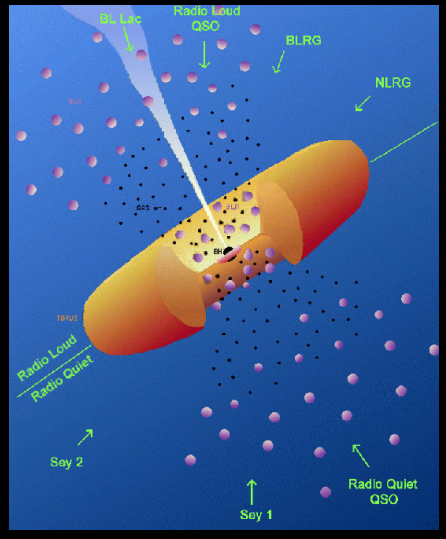
\includegraphics[width=0.6\linewidth]{screenshot_2024-01-26-154109.png}
\end{center}
So all the objects are described by the central black hole being surrounded by an Accretion disk, a broad line region, a dusty torus and a Narrow line region.

\subsection{Apparent super luminous motion}
many of the plumes appear to travel at speeds exceeding the speed of light.

\begin{center}
    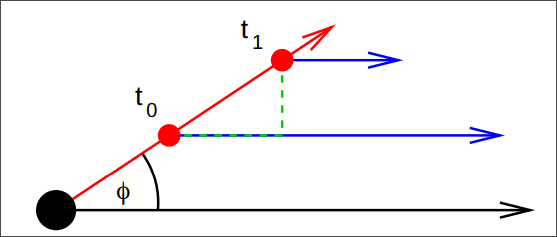
\includegraphics[width=0.6\linewidth]{screenshot_2024-01-26-154432.png}
\end{center}
Consider a blob moving towards us with speed v and angle $\phi$ with respect to line of sight, which
emits signals at $t_0$ and $t_1 = t_0 + \Delta t$ \\ 
Light travel time: The observer sees signals separated by:
\begin{align*}
   \Delta t_0 = \Delta t_e - \Delta t_e \frac v c cos \phi  = (1 - \frac v c cos \phi) \Delta t_e
\end{align*}
The observed distance travel is:
\begin{align*}
   \Delta l = v \Delta t_e sin \phi  
\end{align*}
For small angles we then get:
\begin{align*}
    v_{app }  = \frac {\Delta l}{\Delta t_0 } = \frac {v \Delta t_e sin \phi }{(1 - \frac v c cos \phi)\Delta t_e} = \frac {v sin \phi }{(1 - \frac v c cos \phi)}
\end{align*}
Therefore the observed velocity can be grater than the speed of light. 

\subsection{AGN jets}
\begin{itemize}
    \item most sources appear to be onesided 
    \item The apparent speeds are between 1 and 15 c but can reach up to 50 c
    \item In the same jet the same components tend to have the same speeds
    \item In many sources, bent trajectories are seen, which do not
back-extrapolate to the core: no ”cannon-balls” but patterns in
streaming plasma!
\end{itemize}
At relativistic speeds we also have to consider other relativistic effects. 
The relativistic Doppler factor:
\begin{align*}
    D &= \frac 1 {\gamma (1 - \frac v c cos \phi)} = \frac {\sqrt{1-\beta^2}}{1 - \beta cos \phi}
\end{align*}
The Doppler factor is a strong function of the aspect angle and can become very large for v $\rightarrow$ c.
This factor can become 100 or higher for small angels.

One can show that $S_v / v^3$ is invariant under a Lorenz transform.
Therefore, observed intensity of a moving blob: 
\begin{align*}
    \frac {I (v_{observed})} {v^3_{observed}} = \frac {I (v_{em})} {v^3_{em}}
\end{align*}
and 
\begin{align*}
    I (v_{observed}) = v^3_{observed} \frac {I(v_{em})} {v_{em}^3} = D^3 I (v_{em})
\end{align*}
For a blob with the power spectrum law we then get:
\begin{align*}
    I(v_{obs}) = D^{3-\alpha} I(v_{em})
\end{align*}
Therefore even for small relativistic velocities (e.g. 0.97c) the forward flux can be boosted by a factor of 1000 and the backward flux cut by a factor of 1000.
Therefore: 
\begin{align*}
    \frac {F_1}{F_2} = (\frac {1+\beta cos \phi}{1-\beta cos \phi})^{3-\alpha}
\end{align*}
Even for mildly relativistic speeds and large
angles, features on the approaching side are
always significantly brighter than on the receding side.
One sidedness of jets is a relativistic effect!
AGN slides 42 - end idk look it up.
\section{Large scale structures}
\subsection{Local group}
Around 30 galaxies withing 1 $Mpc^3$.
Centered between the two mayor spirals of the Andromeda (M31) and Milky way galaxies (M33 Triangulum also exists).
Also one major elliptical (M32) around M31.
Apart from that a couple of dwarf and irregular galaxies exist mostly orbiting M31 and the Milky way.
For the brightest objects the distances are known within ~10\% while the distances to the fainter objects are known to a factor of 2. 

The local group is a very topical galaxy cluster. \\ 
The luminosity is dominated by the few brightest members. \\ 
While Andromeda and the Milky way approach each other at around 120 km$s^{-1}$ most others are within 60 km$s^{-1}$. 
Thus the local group is bound gravitationally and wont be ripped apart by expansion.

Observationally around 50 \% of all galaxies can be found in such clusters.
As a general roil of thumb these clusters are: 
\begin{itemize}
    \item a group of galaxies within 1 Mpc
    \item gravitationally bound
    \item for groups the mass is above $10^{13} M_\mathSun$, while the mass of clusters is up to $10^{15} M_\mathSun$
    \item Galaxy groups have less than 50 members with masses up to $10^{14} M_\mathSun$ (mostly spirals and irregulars)
    \item Galaxy clusters have more than 50 members with masses above to $10^{14} M_\mathSun$ (mostly S0 and ellipticals) most of the mass is in hot inter cluster gas
    \item these are cosmologically young structures
\end{itemize}

\subsection{Galaxy interactions}
As two galaxies pass each other part of their energy of motion is transferred to motion of individual stars.
The interacting galaxies are slowed down and may eventually merge.
\begin{align*}
    F_o &= \frac {GmMr}{(r^2+v^2 t^2)^{3/2}} = M \frac{dv_p}{dt}  \\
    \Delta v &= \int \frac {Gmr}{(r^2+v^2 t^2)^{3/2}} dt = \frac {2Gm}{bv}
\end{align*}
The faster the galaxies move, the smaller the velocity change.
This calculation assumes that the galaxies are much smaller than b and that we have a rapid flyby, i.e., M and m do not move during the encounter.
The star m gains an equal and opposite momentum, so the total energy transferred into perpendicular motion is:
\begin{align*}
    \Delta E_{kin,o} &= \frac M 2 \frac {2Gm}{bv}^2 + \frac m 2 \frac {2GM}{bv}^2 = \frac {2G^2m M(M+m)}{b^2v^2}
\end{align*}
The Stellar mass object acquires most of the energy while the Galaxy slows down in parallel direction.
Long before and long after the encounter, the potential energy is small and the energy equation can be expressed solely with the various terms of the kinetic energies:
\begin{align*}
\frac M 2 v^2 &= \Delta E_{kin,o} + \frac M 2 (v + \Delta v_p)^2 + \frac m 2 (\frac M m \Delta v)^2
\end{align*}
Under the assumption that $\Delta v \ll v$:
\begin{align*}
    \Delta v_p &= - \frac {\Delta E_{kin,o}}{Mv} = - \frac {2G^2m(M+m)}{b^2 v^3}
\end{align*}
Finally, integrate over all stars in galaxy 2 (n stars of mass m):
\begin{align*}
    \frac {dv}{dt} = - \int nv \frac  {2G^2m(M+m)}{b^2 v^3} 2 \pi rdr  = - \frac {4\pi G^2(M+m)}{v^2} nm ln \Lambda
\end{align*}
with $\Lambda = \frac {r_{max}}{r_{min}}$. \\
Deceleration of galaxy 2 by the stars of galaxy 1: dynamical friction.
The slower M moves the larger the deceleration.
More massive systems are slowed down more quickly than small systems.
Consequences:
\begin{itemize}
    \item Small galaxies will merge into large ones 
    \item More massive systems are slowed down more quickly than small systems. As a consequence the cohesion of galaxies weakens leading to stars escaping and stellar disks thickening. This might also present a path for spirals to turn into ellipticals
    \item High velocities in clusters prevent the galaxies from merging. Almost all
mergers are observed in groups
\item Close encounters can trigger bar formation and force gas towards the galaxy
center to fuel an active nucleus
\end{itemize}
\subsection{Red shift surveys}
Redshift survey: Survey of (patch of) sky determining galaxy z and position to predefined magnitude or z.
There are multiple kinds of surveys:
\begin{itemize}
    \item 1D-surveys: \\ very deep exposures of small patch of sky, e.g. HST Deep Field,
Lockman Hole Survey, Marano Field 
\item 2D-surveys:\\ cover long strip of sky, e.g., CfA-Survey (1.5 x 100°
), 2dF-Survey
("2 degree Field"), 6dF-survey.
\item 3D-surveys: \\ cover part of the sky, e.g., Sloan Digital Sky Survey.
These surveys attempt to go to certain limit in z or m.
\end{itemize}
1-D surveys produce the Lyman-$\alpha$ forest, which can be used as a distance measure and probe of large-scale structure
\begin{center}
    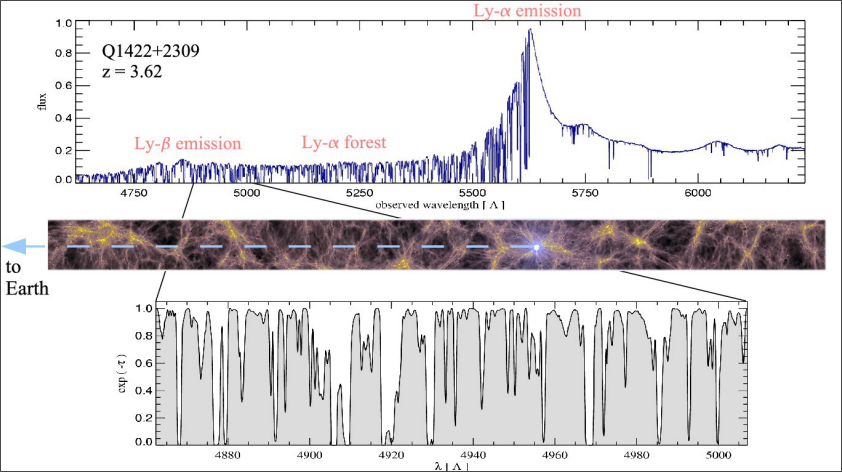
\includegraphics[width=0.9\linewidth]{screenshot_2024-01-27-141853.png}
\end{center}
2D and 3D surveys produce:

\begin{center}
    \includegraphics[width=0.6\linewidth]{screenshot_2024-01-27-142215.png}
\end{center}
\section{Cosmology}
How did the universe evolve to what it is today? \\
There are three basic observations:
 \begin{itemize}
     \item The universe expands
     \item The universe is isotropic
     \item The universe is homogeneous
 \end{itemize}
 Isotropy and Homogeneity form the "isotropic Principal".
 \subsection{Expansion}
 See sec.~\ref{sec:Expansion}
\subsection{Homogeneity}
 
\begin{center}
    \includegraphics[width=0.6\linewidth]{screenshot_2024-01-27-143129.png}
\end{center}
The universe
looks the same, regardless from
where it is observed (On large scales)
\subsection{Isotropy}
\begin{center}
    \includegraphics[width=0.6\linewidth]{screenshot_2024-01-27-143414.png}
\end{center}
The universe looks
the same in all directions.
\subsection{Comoving coordinates}
Mathematical description of the expanding Universe using
"fixed" coordinates ("comoving coordinates"), plus an evolving scale factor R.

Variation of R(t) implies the Hubble constant.
The proper distance is:
\begin{align*}
   D(t) = d_c R(t) 
\end{align*}
As D changes:
\begin{align*}
    \frac {\Delta D}{\Delta t} &=  \frac {R(t + \Delta t)d_c -R(t)d_c}{\Delta t} \\
    \lim_{\Delta t \rightarrow 0} &= \frac {dD}{dt} = v = \dot R d_c = \frac {\dot R} R D = HD \\ 
    \rightarrow H(t) &= \frac {\dot R(t)}{R(t)}
\end{align*}
This leads to the conclusion that the Hubble constant is time dependant. 

The expansion necessarily leads to read shift:
\begin{align*}
    z = \frac {\lambda_{observed} - \lambda_{emitted} } { \lambda_{emitted}} = \frac {R(t_0) - R(t_{em})}{R(t_{em})} \rightarrow \frac { R(t_{em})}{R(t_0)} = \frac 1 {z+1}
\end{align*}
This factor affects two things:  \\
1) convert measured fluxes into intrinsic luminosities L (e.g., distance module), and 2) convert measured angular
scales into linear scales l. The expansion of space affects both conversions, which depend on z!

Define the proper distance $d_p$ as the integral of all infinitesimal path elements
that a photon travels in expanding space from its origin to us.
Then we can calculate the Luminosity: 
\begin{align*}
    d_L &= d_p (1+z) \\ 
    S &= \frac L {4 \pi d_L^2}
\end{align*}
And angular diameter distance:
\begin{align*}
    d_\theta &= \frac {d_p}{1+z} \\ 
    l &= \theta d_\theta
\end{align*}
\subsection{Friedmann Equations}
Equations that describe the time evolution of the scale factor:
Derive dynamics of a mass element on the surface of sphere of density $\rho$(t) and comoving
radius d, i.e., proper radius d · R(t)
Mass of sphere:
\begin{align*}
    M &= \frac {4 \pi} 3 (dR)^3 \rho (t) = \frac {4\pi} 3 d^3\rho_0 \\
    \rho(t) &= \frac {\rho_0}{R(t)^3}
\end{align*}
Force on a mass element:
\begin{align*}
    m \frac {d^2}{dt^2}d R(t) &= - \frac {GMm}{(dR(t))^2} = - \frac {4 \pi G}{3} \frac {d \rho_0}{R^2(t)} m 
\end{align*}
Cancelling md gives the momentum equation:
\begin{align*}
    \ddot R &= - \frac {4 \pi G} 3 \frac {\rho_0}{R(t)^2}= - \frac {4 \pi G} 4 \rho (t) R(t) 
\end{align*}
Multiplying with $\dot R$ and integrating yields:
\begin{align*}
    \frac 1 2 \dot R (t)^2 = \frac {4 \pi G} 3 \frac {\rho_0}{R(t)} + const =  \frac {4 \pi G} 3 \rho(t)R(t)^2 + const
\end{align*}
The constant can only be derived by using GR.
Gr approach: \\
Insert metric into Einstein equation to obtain differential equation for R(t):
\begin{align*}
    R_{\mu v} - \frac 1 2 \mathcal{R} g_{\mu v} = G_{\mu v} = \frac {8 \pi G}{c^4}T_{\mu v} + \Lambda g_{\mu v}
\end{align*}
\begin{itemize}
    \item $g_{\mu v}$: metric tensor ($ds^2=g_{\mu v} dx^\mu dx^v$)
    \item $R_{\mu v}$: Ricci tensor, function of $g_{\mu v}$
    \item $\mathcal R$: Ricci scalar, function of $g_{\mu v}$
    \item $G_{\mu v}$: Einstein Tensor, function of $g_{\mu v}$
    \item $T_{\mu v}$: Stress-Energy Tensor, describing curvature of space due to its field
    \item $\Lambda$: Cosmological constant
\end{itemize}
This is simplified by the Robertson-Walker metric:
\begin{align*}
    ds^2 = R(t)\frac{(dx_1)^2 + (dx_2)^2 + (dx_3)^2} {(1+k' (x_1^2 + x_2^2 + x_3^2)/4)^2} - c^2 dt^2 
\end{align*}
k' describes the curvature of space time and can be -1,0,1. 

In a homogeneous and isotrope universe, the curvature of space is constant throughout all space.

When looking at the energy equation of $\Lambda$ = 0:
\begin{align*}
    H(t)^2 &= \frac {\dot R} {R} ^2 = \frac {8 \pi G \rho (t)}{3} - \frac {kc^2}{R^2}
\end{align*}
And therefore:
\begin{align*}
    k \frac {c^2}{R(t)^2H(t)^2} = \frac {8 \pi G}{3 H(t)^2}\rho (t)-1 = \frac {\rho (t)}{\rho_{crit}} -1 = \Omega -1
\end{align*}
Where $\Omega$ is the density parameter.
$\Omega$ describes the shape of the universe:
If $\Omega > 1 \rightarrow k > 0$, if $\Omega = 1 \rightarrow k = 0$, if $\Omega < 1 \rightarrow k < 0$

The solution to the Friedman equations depends on the boundary conditions. 
These are the value of H measured today and the Density parameter of the universe.
The density parameter is the sum of all matter and the cosmological constant "Dark energy".

Hubble time: 
Assumes an empty universe i.e. Density parameter of 0. 
\begin{align*}
    t_H = \frac v d  = \frac 1 {H_0}
\end{align*}

If the density parameter is larger than 1 then the universe will bounce back onto itself, if its 1 then the expansion will stop at infinity and if its smaller than 1 it will expand forever.
\section{Hot Big bang}
Measurements of the cmb reveal it to be cold ~2.7 K.
CMB photons do however lose energy during universe transversal.
This leads to the conclusion that they had very high energies when they were send out.

$\rightarrow$ Big Bang Theory: Initially, the universe was very hot and as it expanded,
it cooled down.
\begin{center}
    \includegraphics[width=0.3\linewidth]{screenshot_2024-01-28-133552.png}
\end{center}
\begin{itemize}
    \item $10^{-44}s$: GUT \& gravitation: Theory of Everything (TOE)
    \item $10^{-34}s$: electroweak \& strong nuclear force: Grand Unifying Theory (GUT)
    \item $10^{-11}s$: electromagnetic \& weak nuclear
forces: electroweak force
\end{itemize}
after $10^{-11}s$ physics is understood.

At $10^{-4}S $ Temperature cooled down to $10^{12}$K, corresponding to energies of E = $kT$ = 86MeV.
Universe consisted only of a few particle types:
photons, electrons, positrons, neutrinos and anti-neutrinos, as well as a few protons and neutrons ($N_p = 10^{-10}N_{photons}$). 

The primary reactions were:
\begin{align*}
    e^- + e^+ &\leftrightarrow \gamma \\ 
    \gamma &\leftrightarrow v^- + v^+ \\ 
    n + e^+ &\leftrightarrow p + \hat v_e \\
    p + v_e &\leftrightarrow n + e^-
\end{align*}
The resulting thermodynamic equilibrium:
\begin{align*}
    \frac {N(n)}{N(p)} = exp (-\frac{(m_p - m_n)c^2}{kT}) 
\end{align*}
where $(m_p - m_n)c^2$ decrees with T.

At t = 2s Temperature has decreased to $2 \cdot 10^{10}$ K.
This means the end of thermodynamic equilibrium.

Therefore:
\begin{itemize}
    \item (Anti-) Neutrinos freeze out leading to them no longer interacting with other particles
    \item $\frac {N_N}{N_P}$ now 0.223
    \item electron positron pair formation stops the annulation of them leaves very few romancing
    \item no neutrons can be formed anymore, they decay to protons with a half-life of 10.3 minutes 
\end{itemize}
At a time of 230s and temperature of $\cdot 10^{9}$ K:
Deuterium and Helium start forming.

Nucleosynthesis sets in leading to the formation of deuterium, tritium, Helium, lithium.
Their formation is strongly dependent on $\Omega$. 

Stars produce much less hydrogen than is observed. 
This is however explained easily using stellar nucleosynthesis.

This process stops after half an hour.

There are however several problems with the hot bigbang model:
\begin{itemize}
    \item Horizon problem: Why is the CMB so isotropic \\ 
        At the time of decoupling T = 300000 years objects that are now more than two degrees apart could have never have been in causal contact. 
    Nevertheless only very small spacial variations are observed in the CMB.
    \item Flatness problem: why is the density so close to critical i.e. $\Omega$ ~ 1\\ 
        Due to expansion $\Omega$ is changing with time. 
        if $\Omega$ = 2 at time of decoupling of radiation and matter:
        Big crunch after two million years\\ 
        if $\Omega$ = 0.5 at time of decoupling of radiation and matter:
        Very fast universal evolution leading to no stars and galaxies being able to form
    \item Why is there no antimatter 
        Early universe was in thermodynamic equilibrium
 there should have been as much matter as antimatter
But: If there were as much matter as antimatter formed in the Big Bang, they
would have annihilated very soon.
$\rightarrow$ Only photons would have remained, we should not exist.
Observations of Big Bang nucleosynthesis: ratio of hadrons to photons: ~ $5 \cdot 10^{-10}$
$\rightarrow$ slightly more matter than antimatter must have been formed.
$\rightarrow$ There must have been some kind of symmetry breaking in the production of
elementary particles in the very early universe!
    \item What are Dark matter and energy (not explained at all)
    \item If the CMB is so uniform how could stars and galaxies form so early?
\end{itemize}

One possible explanation would be inflation: \\
Basic assumption:
During the big bang there was a phase where $\Lambda$ dominated the Friedmann equation.
For the equation:
\begin{align*}
    H^2 &= \frac {8 \pi G \rho}{3} - \frac k {a^2} + \frac \lambda 3  
\end{align*}
with a dominant cosmological constant we get: 
\begin{align*}
    H(t) &= \sqrt \frac \Lambda 3 
\end{align*}
and 
\begin{align*}
    a = e^{Ht} 
\end{align*}
During inflation, the universe expanded exponentially.
When and why did inflation happen?
Typical assumption: Inflation = phase transition of a scalar field ("inflaton") associated with Grand Unified Theories = GUT.
Universe was so small before inflation that all parts of it were in causal contact.
This inflation would have lasted for 100 Hubble time ($10^{-32}$s). 
This would lead to an expansion of $10^43$

This solution is however constructed.

\section {Determining \texorpdfstring{$\Omega$}{TEXT}}
The evolution of the universe depends on
\begin{align*}
    \Omega = \frac {\rho} {\rho_{crit}} = \Omega_M + \Omega_\Lambda
\end{align*}
Where M is due to gravitating stuff and $\Lambda$ due to exotic stuff.
\subsection{Determining \texorpdfstring{$\Omega_M$}{TEXT}}
\begin{align*}
    \Omega_M &= \frac {\rho_m}{\rho_{crit}} = \frac {8 \pi G \rho_m}{3 H^2}
\end{align*}
For a typical ensemble of stars 
\begin{align*}
   \frac M L = const. 
\end{align*}
we therefore often express $\Omega$ in terms of a mass to luminosity ratio:
Using canonical luminosity density of universe, one can show that
\begin{align*}
    \frac M L = 1390 h \frac {M_{\mathSun}} {L_\mathSun}
\end{align*}
This leads to the conclusion that lots of dark matter exists if $\Omega$ is equal to 1.
$\Omega_M$ consists of: \\
Radiation, Neutrinos (both from early universe), Baryons dark matter. 
The parts of Neutrinos and Radiation are to small to be important. ($\Omega ~ 10^{-5}$)

The parts from matter account for a larger but still insignificant part of 0.043 according to nuclesinthesis.

The mass of galaxy clusters:
Using the viral theorem:
\begin{align*}
    E_{kin}  = - \frac {E_{pot}}{2}
\end{align*}
Assuming isotropy we get: 
\begin{align*}
    <v^2> &=  <v_x^2>+<v_y^2>+<v_z^2> = 3 <v_{||}^2 >
\end{align*}
Assuming the velocity dispersion is independent of $m_i$:
\begin{align*}
    E_{kin} = \frac 3 2 M <v_{||}^2> 
\end{align*}
Where M is the total mass. 
If a cluster is spherically symmetric we can define the wight et mean separation $R_{cl}$ so that:
\begin{align*}
    E_{pot}  &=  \frac {GM^2}{R_{cl}} \\
    \rightarrow M &= \frac 3 G <v^2_{||}> R_{cl}
\end{align*}
Using more complicated models we get
\begin{align*}
    \frac M L = 350 h^{-1} \frac {M_{\mathSun}} {L_\mathSun}
\end{align*}
While we would have expected 10 or 20 from galaxies.
Therefore Dark matter is an important
constituent in galaxy clusters
However Baryonic and dark matter together, make up only ~30 \%
of the critical energy density

X-ray emissions from clusters can be used to determine $\Omega$ to a high percussion and yield: 
\begin{align*}
   \Omega_M = 0.3 \sqrt h 
\end{align*}
Assume gas in potential of galaxy cluster. If gas is in hydrostatic equilibrium:
\begin{align*}
    \frac {dP}{dr} &= - \frac {GM_r \rho}{r^2} 
\end{align*}
With P:
\begin{align*}
    P = nkT = \frac {\rho k T }{\mu m_H} 
\end{align*}
where $m_H$ is the mass of a hydrogen atom and $\mu$ is the mean molecular weight.
Differentiating this leads to: 
\begin{align*}
    \frac {dP}{dr} = \frac {\rho k T }{\mu m_H}  (\frac {d log \rho}{dr} + \frac {d lof T}{dr})
\end{align*}
Combining this leads to:
\begin{align*}
    M_r = -\frac {kTr^2} {G \mu m_H} (\frac {d log \rho}{dr} + \frac {d lof T}{dr})
\end{align*}

Sunyaev-Zeldovich:\\
Gas in clusters influences CMBR by Compton upscattering

The basic ingredients are the optical depth for
Compton scattering
\begin{align*}
    y = \int \frac {kT_e}{m_ec^2} \rho_T N_e dl 
\end{align*}
From this follows in the Rayleigh-Jeans regime
that the intensity due to Compton upscattering
changes as follows:
\begin{align*}
    \frac {\Delta I} I = -2 y = 10^{-4} 
\end{align*}
Therefore we can determine the mass.
This leads to a very similar value of 0.25
Gravitational lensing also agrees with these values:

Therefore $\Omega_\Lambda$ has to be around 0.7

\end{document}
